\documentclass[oneside,9pt]{memoir}

% Colors
\usepackage[dvipsnames]{xcolor}

% hyperref
\usepackage[%
    colorlinks=true,
    linktocpage=true,
    breaklinks=true,
    linkcolor=RoyalBlue,
    urlcolor=RoyalBlue,
    citecolor=RoyalBlue
]{hyperref}
\def\sectionautorefname{§}


% Fonts
\usepackage{fontspec}
\setmainfont[Numbers = {OldStyle, Proportional}]{TeX Gyre Pagella}

\usepackage{amsmath}
\DeclareMathOperator*{\argmax}{arg\,max}
%\usepackage{amssymb}
\usepackage{unicode-math}
\setmathfont{TeX Gyre Pagella Math}

% Typography
\usepackage[tracking]{microtype}

% Images
\usepackage{graphicx}

% ======================================================================
% Memoir package - layout and styling
% ======================================================================

% The calc package is required for calculating readable text widths
\usepackage{calc}

% Set outer and spine margins A wide right margin is chosen both for legibility
% of the typeblock and for tight integration of marginfigures and margin
% footnotes.

% Calculate widths in pts
\setlxvchars[\normalfont\normalsize] % about 66 characters per column
\setxlvchars[\normalfont\footnotesize] % about 45 characters per column

% Set left and right margins
\setlrmarginsandblock{1.15in}{3.5in}{*}
% Set upper and lower margins
\setulmarginsandblock{1.1in}{1.1in}{*}

% Set properties of margin notes, sidecaptioned floats, and footnotes in the
% margin.
\setmarginnotes{0.2in}{2.15in}{2\onelineskip}
\setsidecaps{0.2in}{2.15in}
\sidecapmargin{outer}
\renewcommand*{\sidecapstyle}{\normalfont\footnotesize}
\setsidecappos{c}


% Set footnotes in the margin rather than at the foot of the page
\footnotesinmargin
\setsidefeet{\marginparsep}{1.9in}{0.2in}{0pt}{\flushleftright\footnotesize}{*}

% Integrate the counters of the sidefootnotes and footnotes in margin.
\letcountercounter{sidefootnote}{footnote}
\setlength{\footmarkwidth}{0em}
\setlength{\footmarksep}{-\footmarkwidth}
\setlength{\footparindent}{1em}
\sideparmargin{outer}

\renewcommand*{\sideparfont}{\color{Maroon}\emphshape}
\renewcommand*{\sideparvshift}{2\baselineskip}
\marginparmargin{outer}

% Style the entries in the Table of Contents
\renewcommand*{\cftchapterfont}{\scshape\MakeTextLowercase}
\renewcommand*{\cftpartfont}{\color{Maroon}\scshape\MakeTextLowercase}
\captionstyle[\centering]{\footnotesize}
\captionnamefont{\footnotesize\color{Maroon}}

%% Bringhurst chapter and head styles with a Pedersen-type chapter number
\makechapterstyle{bringhurst}{%
	\renewcommand{\chapterheadstart}{} 
	\renewcommand{\printchaptername}{} 
	\renewcommand{\chapternamenum}{} 
	\setlength{\midchapskip}{15mm}
	\renewcommand*{\printchapternum}{%
        \begin{marginfigure}[0pt]
          \resizebox{!}{\midchapskip}{\color{Maroon}\emph{\thechapter}}
        \end{marginfigure}
      }
	\renewcommand{\afterchapternum}{} 
	\renewcommand{\printchaptertitle}[1]{%
	  \raggedright\Large\scshape\MakeLowercase{##1}}
	\renewcommand{\afterchaptertitle}{%
	  \vskip\onelineskip \hrule\vskip\onelineskip}
}
\setlength{\cftsubsectionindent}{0.6in}
\chapterstyle{bringhurst}
\headstyles{bringhurst}

\tightlists

% Headers and footers - page numbers, section headings, etc.
\makepagestyle{tufte}
\createmark{chapter}{left}{nonumber}{}{}
\makeoddhead{tufte}{}{}{\scshape\MakeTextLowercase{\leftmark}~~|~~\thepage}
\makeevenhead{tufte}{\thepage~~|~~\scshape\MakeTextLowercase{\rightmark}}{}{}
 \makerunningwidth{tufte}[8in]{8in}
\aliaspagestyle{chapter}{empty}
\nouppercaseheads
\pagestyle{tufte}

\checkandfixthelayout

% Bibliography management
\usepackage[%
    backend=biber,
    style=numeric-comp,
    sorting=none,
    natbib
]{biblatex}
\addbibresource{bibliography.bib}

% ======================================================================
% Creating the title page
% ======================================================================

\begin{document}
\thispagestyle{empty}
\begin{center}
    {\LARGE ToMCAT Study 3 Preregistration}\\
    \bigskip
    \textbf{Abstract}
\end{center}

    In this document we declare a number of artificial social intelligence
    (ASI) capabilities being developed for ASIST Study 3 by the ToMCAT (Theory
    of Mind-based Cognitive Architecture for Teams) team. We also declare a few
    offline analyses that we will perform with Study 3 data, with the goal of
    leveraging insights gleaned from the analyses to build ASI components for
    future studies. Given the importance of spoken natural language
    communication understanding for human social intelligence, we place
    significant emphasis on related capabilities.
\begin{center}

    \bigskip

    \textbf{Authors}

    \bigskip

    \begin{tabular}{ll}
        \toprule
        Name & Institution \\\midrule
        Salena Ashton & University of Arizona\\
        Loren Champlin & University of Arizona\\
        John Culnan & University of Arizona\\
        Kobus Barnard & University of Arizona\\
        Emily Butler & University of Arizona\\
        Ruihong Huang & Texas A\&M University \\
        Meghavarshini Krishnaswamy & University of Arizona\\
        Clayton Morrison & University of Arizona\\
        Md Messal Monem & Texas A\&M University \\
        Remo Nitschke & University of Arizona\\
        Adarsh Pyarelal & University of Arizona\\
        Ayesha Qamar & Texas A\&M University \\
        Adam Ussishkin& University of Arizona\\
        Yuwei Wang & University of Arizona\\
        Andrew Wedel & University of Arizona\\
        Liang Zhang & University of Arizona\\
        \bottomrule
    \end{tabular}
\end{center}

\newpage
\tableofcontents* 

\chapter{Introduction}
\textbf{Adarsh Pyarelal}

\section{Purpose and structure}

This document serves the following purposes.

\begin{itemize}
    \item Declare the capabilities we aim to demonstrate for our online agent
        components in ASIST Study 3.
    \item Declare how we will evaluate the capabilities of our online agent in
        ASIST Study 3.
    \item Declare the offline analyses we plan to perform on ASIST Study 3 data
        in advance.
\end{itemize}


The goal of the preregistration process as originally devised
\citep{Nosek.ea:2018} is to separate hypothesis-generating (exploratory)
research from hypothesis-testing (confirmatory) research when Null Hypothesis
Significant Testing (NHST) is used as the evaluation method. A large portion of
the activities engaged in by TA1 performers in ASIST does not fit neatly into
the paradigm either because: (i) the `hypotheses' are about the value of
technological components (e.g., models, algorithms, and systems) for improving
the performance of artificial agents, not about theories about the world (e.g.,
human behaviour) and/or (ii) the evaluation of the evidence for or against the
hypotheses is not doing using NHST.

For this reason, while we endeavor to specify our analyses and capabilities in
as much detail as we can, we do not specify specific social science-style
hypotheses to be tested\footnote{Whether TA1 performers \emph{should} be
    specifying formal, quantitative hypotheses is another discussion.}.

One of the primary motivations for this preregistration document from the
perspective of a TA1 performer team is to accelerate the writing up of
manuscripts for publication by using the structure provided by the
preregistration process to plan ahead for publications.

Each of the sections in this document is a `component preregistation' that
corresponds to a publication `seedling', with the content optimized for what we
call `copy-pasteability', that is, the ability to be copied verbatim into a
manuscript for publication with minimal changes. This is intended to reduce
duplicate effort between writing up preregistrations and publications.

Since our team is relatively large, there is little overlap in the author lists
for the individual component preregistrations. Thus, each component
preregistration has the names of the primary authors responsible for its
content section displayed under its title heading in addition to the table at
the beginning of this document. Authorship is ascribed to those who have
contributed substantially to the ideation or writing of the content.

\section{Overview}

Broadly speaking, we are aiming to develop a suite of open-source technologies
for artificial social intelligence, with a focus on computational understanding
of spoken team dialogue. Each of the component preregistrations demonstrates a
capability that we believe is important for artificial social intelligence, and
is currently integrated or will be integrated in the near future into our ASI
agent that will be evaluated in ASIST study 3 or future ASIST experiments.

For ASIST Study 3, we will deploy three Dockerized components. Two of them can
be classified as `analytical components' (ACs) in the parlance of the ASIST
program, and one as an `ASI', i.e. an AI agent imbued with artificial social
intelligence. The current delineation between ACs and ASIs has been made based
on container boundaries. In principle, the two ACs devoted to speech and
natural language processing (see \autoref{fig:nlp-architecture}) could be
bundled and deployed as part of our ASI, but we opt to keep them separate as we
expect that the resulting modularity will be beneficial for future
applications.

\begin{figure}
    \centering
    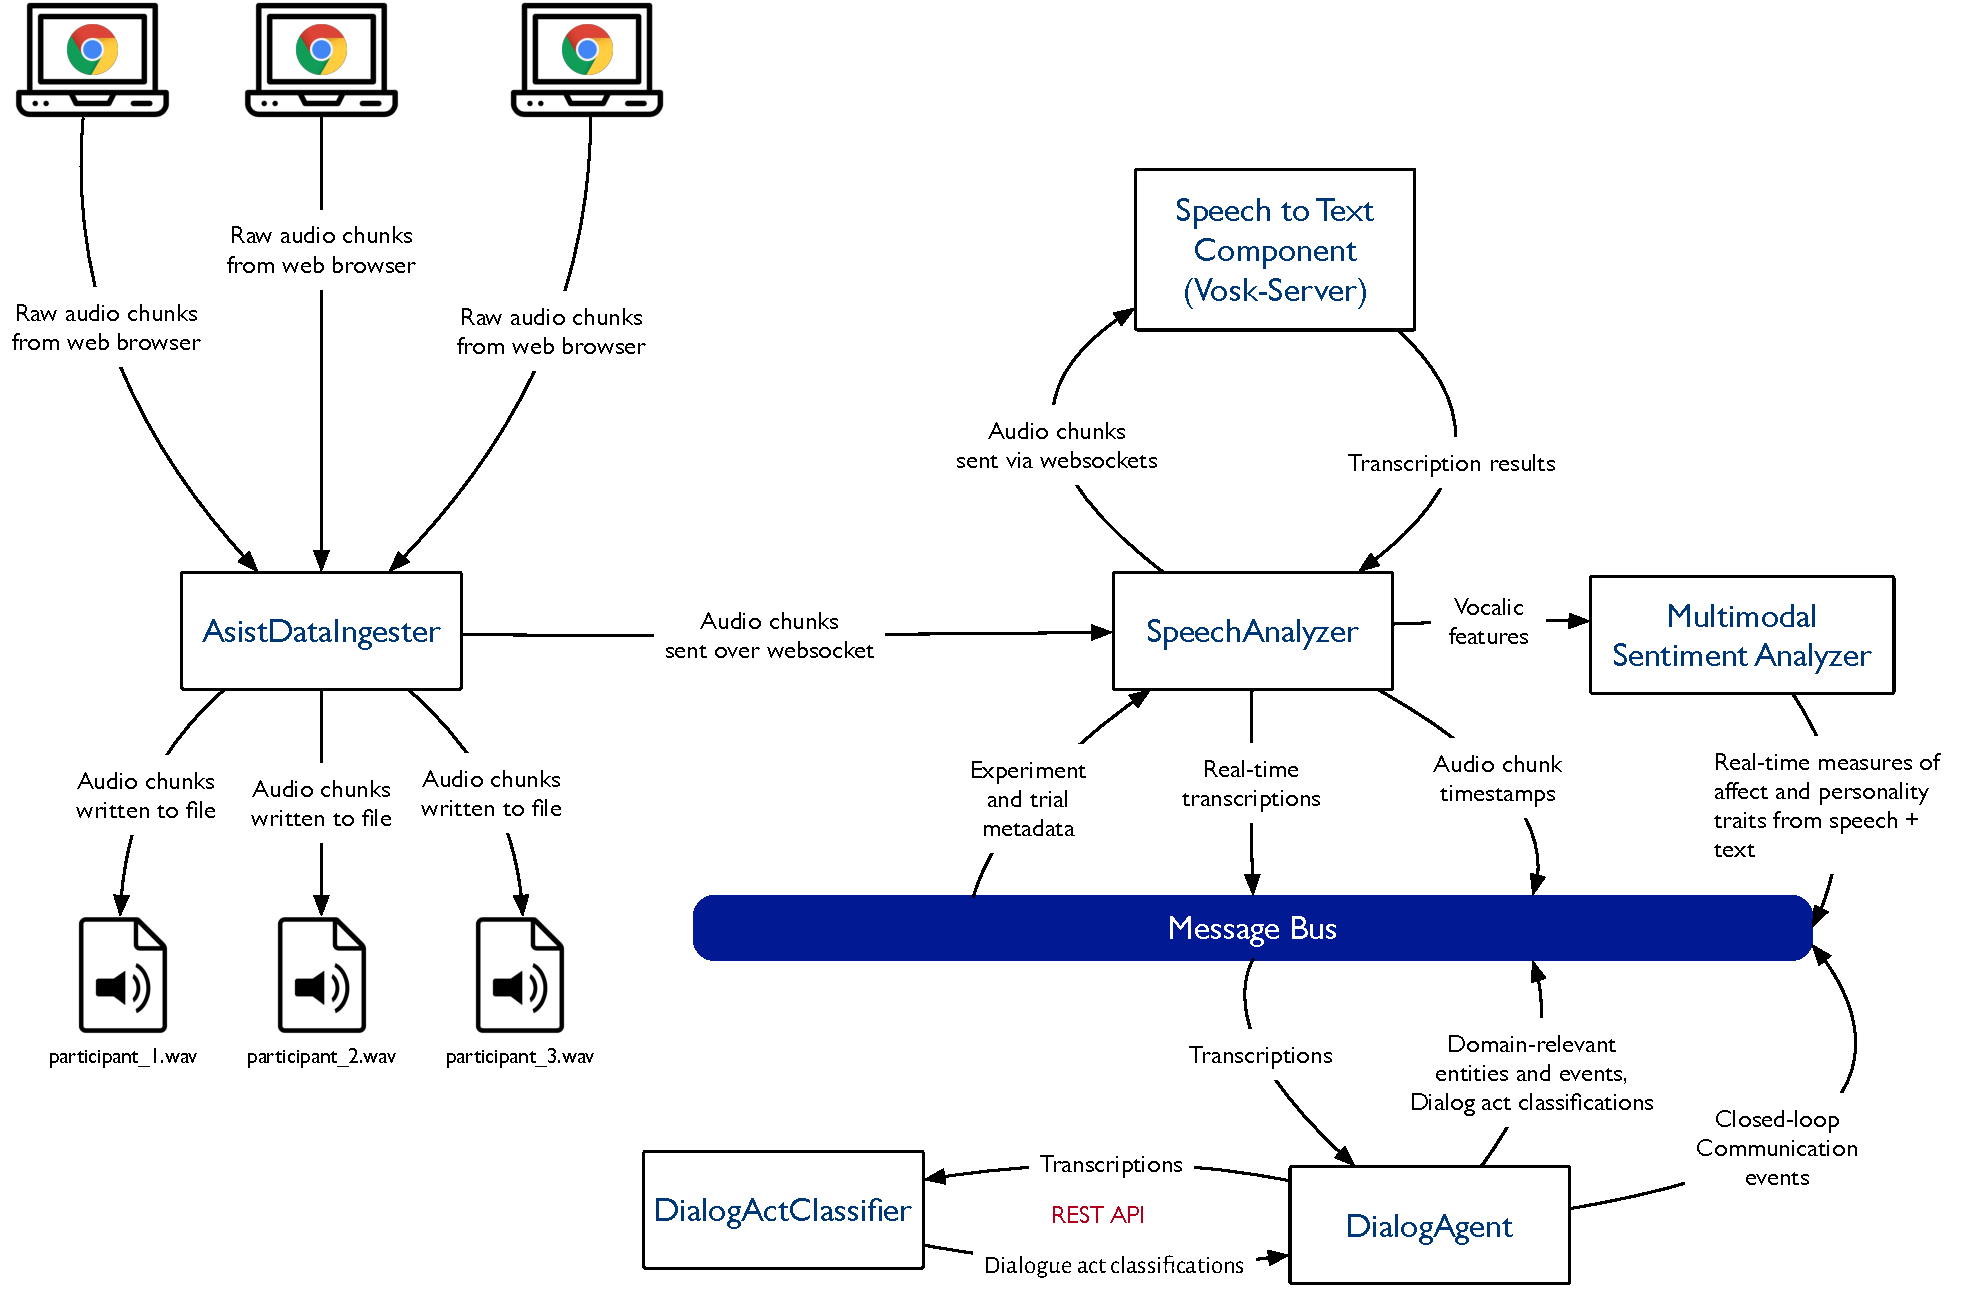
\includegraphics[width=6.5in]{images/nlp_architecture}
    \caption{Architecture of our multi-participant dialogue analysis system.}
    \label{fig:nlp-architecture}
\end{figure}

%Give a brief summary of the preregistrations and how they contribute to the overall architecture.

The component preregistrations in this document span a broad spectrum of
research topics, but work together to form a cohesive suite of ASI
capabilities.

Chapters \ref{ch:rule_based_ie} and \ref{ch:sentiment_analysis} focus on
gleaning information from individual natural language utterances. Chapter
\ref{ch:rule_based_ie} discusses our rule-based system for extracting entities
and events from natural language text, and \autoref{ch:sentiment_analysis}
describes our approach to detecting sentiment and personality traits using both
text and speech information.

In chapters \ref{ch:da_classification} and \ref{ch:clc}, we move
beyond analyzing utterances individually to analyzing them \emph{in context},
that is, we consider windows containing multiple utterances to detect
longer-range phenomena. Chapter \ref{ch:da_classification} uses context to identify
dialogue acts, and \autoref{ch:clc} uses it to automatically detect
closed-loop communication. Chapter \ref{ch:da_classification} also discusses
using multiple modalities (speech and text) to classify dialogue acts.

In \autoref{ch:entrainment}, we discuss our approach to detecting real-time
conversational alignment, or \emph{entrainment} between teammates. In
\autoref{ch:plan_recognition}, we describe our approach to multi-agent plan
recognition. The analyses described in this chapter will be performed offline
for ASIST Study 3, but we expect them to be integrated into online components
for ASIST Study 4 and future experiments.

Finally, we describe our probabilistic modeling approach to machine theory of
mind (MToM) and machine theory of teams (MToT) in \autoref{ch:pgm}, along with
our planned interventions in ASIST Study 3 and their rationale.

\label{ch:rule_based_ie}
\textbf{Remo Nitschke}

\section{Introduction}

For humans, verbal and non-verbal communication are insightful indicators of
social processes. Within the scope of ASIST, team-building and communication
within teams is of heightened interest. We maintain, that in order to develop a
model of human agents and human teams, surveying verbal communication is
essential. Our DialogAgent is designed with this goal in mind: Extract
information from player dialog that can be useful in order to create a model of
the player's mental state.

An AI agent needs to formulate a model of the humans and teams it advises. In
order to construct such a model, language data provides essential insights. As
raw natural language data is ``messy", we believe it is necessary to
pre-process and vet this data into chunks that are informative and pertinent to
the AI. This is done via our DialogAgent which provides Dialog Act Labels and
Event Extractions for player utterances. The Dialog Act Labels inform on the
\emph{type} of utterance, whereas the Event Extractions inform on the semantic
\emph{content} of the utterance. In this section we discuss the engine that
constructs the Event Extractions.

\section{Approach}

%% Note to Adarsh: I think we could insert the diagram from Study 2 prereg here (page 2)

Raw communication audio captured during the experiments is processed through
our SpeechAnalyzer which provides transcriptions (transcriptions:
MinecraftEntity\_Observation\_Asr\_Speechanalyzer). The transcriptions are run through our DialogAgent which contains an extensive rule-based event extraction system (ODIN) \citep{valenzuela-escarcega-etal-2016-odins}. Much of modern information extraction and event extraction is done via neural nets, see \citet{Ahmad2021GATEGA,Du2020EventEB}. We are opting for a rule-based system because:

\begin{enumerate}
 \item It allows us to be more flexible with our extraction labels. We can quickly add or remove labels if we see the need to do so.
 \item It allows for high precision for the labels we are interested in. Rules can be crafted to be precise (albeit at the cost of coverage).
 \item Rules do not require us to create, maintain, and annotate extensive datasets. This is especially pertinent within the scope of ASIST, as domain specific terms can change between Studies. It would be near impossible for us to train a neural agent on the new terms of the next study before the data is published.
\end{enumerate}

Our rule based framework returns nested labels and their spans. The nesting of labels represents the argument structure of the event. The extracted events are returned as JSON objects (event extractions: MinecraftEntity\_Event\_Dialogue\_Event\_Dialogagent). 


\subsection{List of Variables}
\begin{itemize}
    \item Input Variables
    \begin{itemize}
        \item transcriptions: MinecraftEntity\_Observation\_Asr\_Speechanalyzer
        %the following only if we want idc in pre reg:
        %\item location data: MinecraftEntity_Event_Location_Locationmonitor
        % \item triage status: MinecraftEntity_Event_Triage_Simulator
        %\item rubble interaction: MinecraftEntity_Event_Rubbledestroyed_Simulator
    \end{itemize}
    \item Output Variables
    \begin{itemize}
        \item Event Extractions: MinecraftEntity\_Event\_Dialogue\_Event\_Dialogagent
    \end{itemize}
\end{itemize}


\section{Evaluation}
We will evaluate via manual evaluation by human annotators. We will hire human annotators to evaluate a representative chunk of utterances. As the DialogAgent currently extracts 100+ labels, we have narrow down this selection in order to avoid overwhelming our annotators. 
We will select 20 labels for annotation. These labels will be selected for two qualities:
\begin{enumerate}
\item Complexity: The DialogAgent labels can be divided in two types. Labels which are generated by string-pattern matching and labels which are generated by a combination of pattern matching, dependency parsing, and tagging. We will call the latter ``complex", as they involve reliance on a dependency parse and are more unpredictable due to the fact that they rely on multiple conditions to trigger. For this evaluation, ``complex" labels are more pertinent, as their accuracy is harder to predict. \footnote{A brief explanation as to why ``simple" labels are less interesting. Assume a label for players talking about ``victims". This label will be generated by a simple pattern matching rule that scans all tokens for a regular expression looking something like this: {/(?i){$\hat$ }victims?\$/}. This pattern will match any and all occurrences of ``victim" (plural or singular). The precision and recall of this label now depends entirely on the quality of the transcript and on the way the players talk about ``victims" (for example, they may use other terms as well). This makes this label much more predictable, than one that relies on dependency graphs in addition to pattern matching.}
\item High Frequency: The selected label should be sufficiently high in frequency to generate a representative amount of data. As our labels are often very specific, and thus rare, we will circumvent this issue by letting annotators annotate for groupings of labels.\footnote{For example: We have five different labels for players ``needing something", such as a specific item, a specific role, or just help from other players. In order to lighten the load on annotators, we will subsume these under one label.}
\end{enumerate}

Annotators will receive transcripts of player communications. They will be asked to annotate the transcripts for the 20 labels we have giventhem. With this annotated data, we can write a script that will counter-check the DialogAgent extractions against the annotations and calculate a representative F1 score.



\subsection{Precision Evaluation for the Entire Label-Set}
We will also run a seperate evaluation for precision,\footnote{For reasons of economy, we restrict this evaluation to precision. Our expert team-members can judge produced labels for precision at a much higher speed than they can annotate utterances for labels.} done by team members and hired annotators who are familiar with our DialogAgent labels.

We have done a preliminary evalution of this type already, and have found \ldots [NUMBERS HERE]

\subsection{Potential Evaluation Problems}
By subsuming multiple labels under one label for the general evaluation, we run the risk of having no way of discerning if one label in a group is a particularly weak performer. For example, assume we have five different labels for types of questions. Assume we subsume them under one generic ``Question" label for this evaluation. After the annotations are done, we calculate an F1 score for this new label. If one of the five labels was a weak performer (for example, .3 F1), but the others performed well, then the overall F1 score for this label will mask this fact. 

In order to combat this problem, we will run an evaluation for precision over the entire label set, as described in the previous subsection. Unfortunately, we will not be able to generate recall for the entire label set, as this process is simply too costly for 100+ labels.


\chapter{Sentiment analysis and personality trait detection}
\label{ch:sentiment_analysis}
\textbf{John Culnan, Adarsh Pyarelal}
\section{Introduction}

Personality trait detection, sentiment analysis, and related measures of
personal characteristics like emotion recognition\ap{Are we doing sentiment
analysis or emotion recognition? These terms seem related, so we should be
careful to minimize ambiguity. Can you provide definitions?} are all frequently
used to characterize an object of study. As such, they provide an AI agent with
information about the background and states of individuals at any given time,
which may be used to allow the agent to interact with individuals in a manner
appropriate to their current state. Because understanding the personalities and
emotional states of other individuals is a key feature of collaboration among
people, it is a critical component of the identification of the overall mental
states of others as required for a machine theory of mind
\cite{Rabinowitz.ea:2018}. Providing an AI agent with this capability will
likewise help inform a machine theory of teamwork by allowing the AI agent to
incorporate a wider range of key information in performing its own role.

There are no existing state of the art (SOTA) models for the Study 3 dataset, as the
data collection has not been completed yet; however, SOTA models
exist for related datasets and tasks, some of which are incorporated into our
model as task-specific training data. For the Multimodal Emotion Lines Dataset
\cite{Poria.ea:2019}, which consists of a sentiment analysis task and a
discrete emotion recognition task\ap{This is a bit confusing - the dataset
consists of tasks? Should the tasks not be independent of the dataset?}, the
SOTA model is TODKAT \cite{Zhu.ea:2021}, which uses context-aware
text and audio transformer-based models for the emotion recognition task. The
First Impressions V2 dataset \cite{Ponce-Lopez.ea:2016}, consisting of the Big
Five personality trait classification for YouTube clips, was originally created
for use with a regression task\ap{Do we need to mention the original purpose
here?}; as a dominant trait classification task, the
SOTA model is \citet{Culnan.ea:2021}\ap{The wording here seems
strange - `as a dominant trait classification task' - should this be instead
something like `for the task of classifying the dominant personality trait'
instead?}. The Multimodal Opinion-Level
Sentiment Intensity (MOSI) dataset \cite{Zadeh.ea:2016} consists of single
speakers in YouTube clips providing opinions that are rated from highly
negative to highly positive. The current SOTA model for MOSI is
TupleInfoNCE \cite{Liu.ea:2021}, which uses contrastive learning on augmented
data. 

One major limitation of current SOTA approaches is that the data on which they
are trained is not varied in source; typically, each task is trained
separately, so that when two or more tasks have similar or identical label
spaces, the model is retrained for each new task. The data within a given task
generally includes speakers with the same native language.  Multi-party data
furthermore frequently come from scripted sources, such as the television show
Friends \cite{Poria.ea:2019, Zhu.ea:2021}), and single party data from YouTube
\cite{Zadeh.ea:2016, Ponce-Lopez.ea:2016}). Finally, these SOTA models are
created around datasets that rely on accurate, hand-crafted transcriptions of
the audio data, without considering imperfections in the transcriptions. We
approach this challenge by examining the Study 3 data through multitask neural
networks that make use of both existing corpora as pre-training data as well as
the Study 3 data to perform the same tasks in a new domain, further seeking to
improve performance by giving special consideration to the imperfection of
automatic ASR transcriptions used with the Study 3 data\ap{This sentence seems
rather long. Can you split it in two?}. 


\section{Approach}

Our approach includes a hard parameter sharing multitask model pre-trained on
tasks for sentiment \citep{Zadeh.ea:2016}), emotion \citep{Poria.ea:2019}),
personality \ap{personality or personality trait?}\citep{Ponce-Lopez.ea:2016}),
and emotional intensity \citep{Livingstone.ea:2018}), then trained on data from
Study 3. Like \citet{Liu.ea:2021}, our model will make use of augmented data to
allow for more balanced classes in each dataset of interest.  Acoustic and text
data will be fed into the model separately, with text data masked to handle
noise created by automatic transcription. These text transcriptions will be
paired in an ensemble with predictions made by a trained wav2vec model
\citep{Schneider.ea:2019}, which will allow for further boosting of text
modality accuracy. Acoustic and text data will subsequently be concatenated
prior to making predictions about the classes for each utterance-level data
point. A schematic representing our approach is shown in
\autoref{fig:sentiment_model_schematics} \ap{Add more detail in the figure
    caption. In general, figure captions should be somewhat
self-contained and fairly detailed since they will often be the first (and
sometimes only) thing readers look at.}. 

\begin{figure}
    \begin{sidecaption}{%
        Schematic representation of our multitask model
    }[fig:sentiment_model_schematics]
    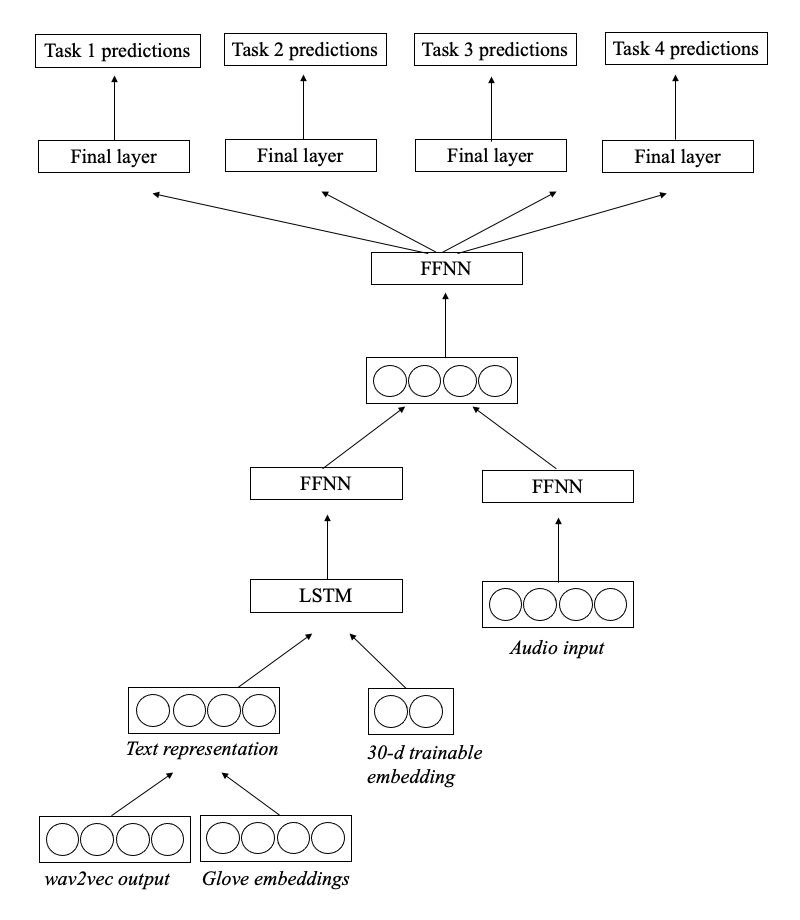
\includegraphics[width=\textwidth]{images/sentiment_schematics_study3.png}
    \end{sidecaption}
\end{figure}

The experiments we propose to run with our model are based on an initial
analysis of two versions of our existing model's results on a subset of the
Study 3 Spiral 3 pilot data. In this initial analysis, we compared models
trained with and without information about the distribution of class labels
\ap{From which dataset? MELD or Study 3 Spiral 3 pilot?}
(i.e., class weights).  For the Study 3 Spiral 3 pilot data, the model trained
with class weights achieved an F1 score of 58.78 for emotion recognition
(comparable to the score achieved on the test partition of MELD \ap{Provide the
acronym expansion and the relevant citation}). However, the model trained
without class weights performed better, reaching an F1 score of 72.64.

For dominant personality trait identification, the results similarly showed
improvement when the model did not include class weights (F1 of 21.58 for Study
3 Spiral 3 data with class weights, F1 of 37.65 for this data without class
weights). These scores were calculated by using annotations for emotion and
sentiment \ap{Again, emotion and sentiment seem semantically similar - hence
the need for definitions in the introduction section.} by two researchers on
our team as gold labels, as well as TIPI \ap{What is TIPI?} survey results for
personality trait identification gold labels. \ap{Can you add tables with these
numbers for quicker scanning?}

Results of both tasks may not have been representative of the true performance
of the model, as the Spiral 3 data used confederates (i.e., members of the
research team) rather than naive participants; it is possible these
participants did not respond to the TIPI in the same way that naive
participants would have, and this group of pilot participants may have been
calmer or more neutral in their speech due to their previous experience with
the missions and data collection procedure. To determine whether this is the
case, data from Study 3 will need to be annotated, with results from a portion
of Study 3 participants compared to the results of Spiral 3
participants\footnote{While data was collected from a set of naive participants
prior to the drafting of this preregistration, this data did not include the
necessary vocalic features for our analysis, due to technical issues. We expect
that the rest of the Study 3 data will contain these features.}.

Furthermore, while the model trained without use of information on the distribution
of gold labels in the training datasets outperformed the model trained with this
information, the model without distributional information did not make predictions
for all possible emotions and traits. In order to rectify this and attempt to
further improve the quality of model predictions, the distribution of data points
across all emotions and traits in the ASIST-specific data rather than pretraining
datasets will be incorporated into this model, as such information may provide an
additional boost to model performance.

The Study 3 data that will be incorporated into our models are the
pre-experiment TIPI survey
(Participant\_CognitiveTenItemPersonalityInventory\_Survey\_PreExperiment), the
text output of the ASR system
(MinecraftEntity\_Observation\_Asr\_Speechanalyzer), the audio data and the
acoustic features extracted from this audio signal
(MinecraftEntity\_Observation\_Audio\_Speechanalyzer)\ap{Convert this to a
bullet point list}. In addition to this previously collected data, new
utterance-level annotations will be collected for sentiment, emotion, and
emotional intensity \ap{Make sure these are defined in the introduction
section}. The text output of the ASR system and the acoustic features extracted
from the audio signals will be used as input data in the model, while the TIPI
and new utterance-level annotations will be used as gold labels to evaluate the
performance of our model. 

\section{Evaluation}

System evaluation will consist of examinations of the network's ability to make
correct predictions about sentiment, emotion, and personality traits using F1
scores calculated by comparing network predictions with survey responses and
human-annotated data as described above. To provide comparable scores to
existing models for these tasks, average F1 scores will be used, calculated as
the weighted average of the F1 score for each class in the task.  Bootstrap
resampling (citation)\ap{Add citation} will be used to provide statistical
comparisons among models created with this network\ap{What is the difference
between `network' and `model' here? I (and maybe other readers) may conflate
the two terms.}, enabling the identification of the best model. 

While F1 calculations provide information on the overall success rate of our
network, they are limited in their ability to identify areas of weakness. To
further evaluate the ability of our network \ap{Again, network or models? Which
is the word `perform' associated with?} to perform under the different
conditions available, a subset of incorrect data points will be examined.
Patterns of errors that demonstrate model weaknesses with a particular type of
data (such as difficulty in correctly identifying neutral sentiment in male
voices) will be used to inform further iterations of network updates. 

\chapter{Closed-loop communication detection}
\label{ch:clc}
\textbf{Yuwei Wang}

\section{Introduction}
Good teamwork and communication enable a group of team agents (which could be human or non-human AI agents) to perform beyond the sum of their parts\citep{roberts2022state}. Especially during high-stakes crisis situations, miscommunication is a common cause of adverse events\citep{taylor2014description}\citep{davis2017operative}. Closed-loop communication(CLC) is often recommended in the team research literature (military and medical communication and training) as a communication behavior that can guarantee the accuracy of information exchange\citep{marzuki2019closed}. Currently, CLC in spoken dialogue is identified via retrospective analyses involving manual transcription and annotation. However, given the potentially catastrophic consequences of poor team communication\citep{flin2004identifying} - especially in complex, fast-paced, and high-stakes environments such as urban search and rescue scenarios - we argue that there is an urgent need for AI technologies that can detect and repair the breakdowns in CLC as they happen. To address this need, we propose to develop an AI system for detecting the presence or absence of CLC procedures in spoken dialogue within teams of humans collaborating on shared tasks.
Currently, most real-time natural language understanding(NLU) and responding systems(e.g. Question and answering\citep{hawkins2017you}, incremental decision-making\citep{devault2011detecting}) are limited to conversing with a single human at a time. On the other hand, there are numerous analyses of multi-participant spoken dialogue in the academic literature - however, their analyses are primarily performed offline rather than in real-time. 
The dialogue system we are building in the Theory of Mind-based Cognitive Architecture for teams(ToMCAT) project addresses both of these limitations. The existing ToMCAT speech analyzer is currently able to analyze spoken conversations in real-time to extract entities and events of interest with a powerful rule-based framework\citep{valenzuela-escarcega-etal-2016-odins}, classify dialogue acts, and detect sentiment. We propose to extend this system to detect closed-loop communication as well. We will start by implementing a set of rules in the module to detect multi-parties CLC procedures. Taking the Study 3 data as the training and developing dataset, we will be able to revise our detection rules and build a CLC detector for real-time conversations.

\section{Approach}
In closed-loop communication protocol, there are three distinct phases\citep{Hargestam.ea:2013}(\autoref{fig:clc-three-phases}, \autoref{tab:clc-three-phases}): 
\begin{itemize}
    \item The sender initiates a message (the Call-out phase).
    \item The receiver acknowledges the message, usually by paraphrasing or repeating the main information of the message (the Check-back phase).
    \item The sender verifies that the message has been received and interpreted correctly(Closed-loop).
\end{itemize}

%\begin{figure}
%    \centering
%    \includegraphics[width=2.5in]{images/clc-three-phases}
%    \caption{Three phases of closed-loop communication}
%    \label{fig:clc-three-phases}
%\end{figure}

\begin{table*}[tb]
\centering
\begin{tabular}{lll}
    \toprule
    Role & Utterance & Phase \\\midrule
   Green & “This is Green. I’m finishing this side, blue, could you check the central for victims?” & Call-out\\
   Blue & “This is Blue. Okay. I’ll go check the central for victims.” & Check-back\\
   Green & “All right, thank you, Blue.” & Closed-loop\\
    \bottomrule
\end{tabular}
\caption{An example of the three phases of closed-loop communication. This example is extracted from Study2 data, while Green is the sender of the request message, and Blue is the receiver of the request message.}
\label{tab:clc-three-phases}
\end{table*}

We are going to develop a procedure to dynamically detect the three phases of CLC. First, the Call-out phase will be detected by rules in our speech analyzer, labels including HelpRequest, Instruction, and NeedAction are used as triggers for Call-out. Next, we examine five utterances followed by other team members. If we find acknowledgement by other team members as well as the same semantic labels as in the Call-out message, then this indicates there is a Check-back phase. Finally, within five utterances following the Check-back, if we see the sender verified the information of the Check-back with the Agreement label, we can determine that this is a closed-loop communication. The triggers and argument rules of CLC detection are illustrated in \autoref{tab:clc-triggers-labels}, and an algorithm for CLC detection is shown in Algorithm 1.

\begin{table*}[tb]
\centering
\begin{tabular}{lp{1in}lll}
    \toprule
    Role & Utterance & Trigger Rules: mentioned text & Argument Rules: mentioned text & CLC label \\\midrule
   Green & “This is Green. I’m finishing this side, blue, could you check the central for victims?” & Instruction: could you check & Action: check \newline Location: central \newline Victim: victims & 1a\\
   Blue & “This is Blue. Okay. I’ll go check the central for victims.” & Agreement: okay & Action: check \newline Location: central \newline Victim: victims \newline Blue:blue & 1b\\
   Green & “All right, thank you, Blue.” & Agreement: All right &  & 1c\\
    \bottomrule
\end{tabular}
\caption{The trigger and argument rules of CLC detection}
\label{tab:clc-triggers-labels}
\end{table*}
\subsection{List of Variables}
\begin{itemize}
    \item Input Variables
    \begin{itemize}
        \item transcriptions: MinecraftEntity\_Observation\_Asr\_Speechanalyzer
    \end{itemize}
    \item Output Variables
    \begin{itemize}
        \item Event Extractions: MinecraftEntity\_Event\_Dialogue\_Event\_Dialogagent
    \end{itemize}
\end{itemize}

\begin{algorithm}
\caption{The algorithm for CLC detection}\label{alg:CLC}
\begin{algorithmic}[1]
\State $CLC-labels \gets []$
\Function{CallOut}{utterance} 
     \If{any(label in [‘HelpRequest’, ‘NeedAction’, ‘Instruction’] for label in $utterance$}
     \State $CLC-labels \gets 1a$
     \EndIf
     \EndFunction

\Function{CheckBack}{utterance} in range (5)

    \If{'Acknowledgement' in labels of next $utterance$
     \If{any(label in CallOut.arguments for label in next $utterance$}
        \State $CLC-labels \gets 1b$
        \EndIf
        } else
    \State $CLC-labels \gets 0.5b$
    \EndIf
    \EndFunction
\Function{CloseLoop}{utterance} in range (5)
     \If{'Acknowledgement' in labels of next $utterance$}
     \State $CLC-labels \gets 1c$
     \EndIf
     \EndFunction
\end{algorithmic}
\end{algorithm}

\section{Evaluation}
The performance of the closed-loop communication detector will be evaluated by human annotators. Annotators will be trained to evaluate the automatically extracted CLC dialogues with the CLC coding scheme in Table 2. For a weak check-back that only acknowledge the call-out with the ‘Agreement’ label but no repeating information is found, the check-back should be labeled as ‘0.5b’ instead of the complete check-back label ‘1b’.
The inter-rater reliability of the annotators will be measured using Cohen’s kappa. When the percentage of agreement between annotators reaches 80\%, and K>.70, annotators could start work on the formal annotation of the data. The precision and F1 score will be used to evaluate the performance of our CLC detector. We will improve the detecting rules and algorithms according to the evaluation. The precision should reach a minimum of 90\% and F1 reach a minimum of 80\% after improvement on the CLC detector has been fully applied.



\chapter{Dialogue act classification}
\label{ch:da_classification}
\textbf{Ruihong Huang, Ayesha Qamar, Messal}

\section{Introduction}

In the Theory of Mind-based Cognitive Architecture for Teams (ToMCAT) project,
we are working on building an AI agent that will assist the players by taking
their speech and facial expressions as input. Speech being a core part of the
inputs, the agents will need to be capable of natural language understanding to
process the conversations to make informed and prompt decisions. Identifying
Dialog Acts (DA) is one of the primary aspects of natural language
understanding. dialog Act (DA) can be identified as a method of defining the
semantic content and communicative function of a single utterance of dialog
\citep{Searle:1969}. Examples include request, question, acknowledgment etc.
Dialog acts can provide important information about the user dialog turns and
set of possible system actions, and the frequencies and patterns of DAs spoken
by different speakers could also potentially indicate the roles they play such
as leader, follower etc., Thus, it is a useful capability for this AI agent and
many conversational agents in general.

Acknowledging the importance of DA classification in natural language
understanding, extensive research has been conducted on DA classification.
These research works have taken different approaches in terms of dataset,
machine learning model and input to the models. The most popular datasets that
are being used are Switchboard Corpus (SwDA) and ICSI Meeting Recorder Dialog
Act Corpus (MRDA). Most of the approaches use textual utterances from dialog
transcripts as input to the model. Statistical machine learning models such as
Support Vector Machines (SVMs) \citep{Henderson.ea:2012}, Hidden Markov Models
(HMMs) \citep{Stolcke.ea:2000}, Conditional Random Fields (CRFs)
\citep{Zimmermann:2009} are employed for identifying DAs. Deep learning models
are also gaining popularity in DA classification. \citet{Liu.ea:2017} presented
both CNN models and hierarchical CNN+CNN and CNN+RNN models to classify dialog
acts and showed that RNN/Bi-LSTM on top of CNN model performs better than other
models in consideration. \citet{Shen.ea:2016} presented that Neural Attention
Model with context information performed well on the SwDA dataset.
\citet{Raheja.ea:2019} achieved state-of-the-art result using context-aware
self-attention model on MRDA corpus. Another approach for DA classification is
incorporating both lexical and acoustic features. \citet{Ortega.ea:2018} showed
that their Lexico-Acoustic neural network models can outperform the similar
models taking only lexical information as input.

Even though these approaches provide excellent results on DA classification,
they lack in various aspects. First of all, most of these models require clean
transcripts as input. Achieving clean transcripts requires manual annotation,
which is both time consuming and costly. As a result, DA classification in real
time is not possible. Another limitation is the lack of explicit addressing to
multiparty dialogs where mechanisms to incorporate speaker identification and
determining the discourse structure is also crucial. Apart from these
limitations, these approaches often use only 5 types of high level tags for DA
classification, which do not entirely explain the DA under question. It is
necessary to have both general and specific tags to completely understand a DA.

We are going to develop a Deep neural network based DA classifier to process
the input utterances in real time which is more aligned with the main goal of
the project that is building an AI agent to be an effective teammate of a
Minecraft player. As the players will play online simultaneously, the agent
needs to understand the conversations of the player as the game progresses. For
the agent to be real time, we cannot rely on manual transcription. Instead we
have used a publicly available Automatic Speech Recognizer (ASR), named Google
Cloud Speech API to convert the utterances into text. This provides noisy text
in return which might harm the performance of the DA classifier. To compensate
for this, we will use acoustic features from the raw speech as well.

\section{Approach}
A Bi-LSTM based baseline model is already trained with clean transcripts. The
same model is trained again with the ASR generated transcripts and the
performance dropped significantly due to ASR noise and the highly overlapping
nature of the utterances in the meetings. To overcome this drop we will use a
fusion based audio-language model to leverage both lexical and acoustic
information of the utterances to successfully identify the DAs. In addition,
our approach will capture the threading structure within a dialogue that
involves detecting utterances falling within an adjacency pair (consisting of a
question and an answer utterance, or a request and an acceptance utterance) and
then linking them together. We will aim to eventually jointly learn both the
threading structure and DAs of a dialog in a multitask learning setting since
we expect the two tasks to benefit each other.

Currently we are using a multi-party dialog dataset MRDA
\citep{Shriberg.ea:2004} that consists of 75 meetings each about an hour long,
where each utterance has one (out of 11) general and zero or more (out of 40)
specific tags. Once the experimentation is done, we will use a transfer
learning approach to train and test the model for study-2 data. 

\section{Evaluation}

To evaluate our approach, we will use F1 score as the evaluation metric. For
multiclass classification problems, especially where the classes are highly
imbalanced, F1 score provides more insight than accuracy.  We also intend to
annotate ASIST data for dialog Acts so that the system trained on MRDA can be
finetuned on ASIST. fine-tuned on ASIST. The baseline model that we are currently 
using is a sequential model consisting of a hierarchical LSTM. The macro F1 score 
for this model on MRDA data is 40.77. However, when we evalute the trained model 
on ASIST study 3 data, the accuracy and F1 score both degrade. The performance of 
the model on raw ASIST data in terms of accuracy and macro F1 score is 30\% and 
9.705 respectively. One of the key factors behind this performance degradation is 
noisy transcripts generated by the ASR. In order to solve this issue we have to 
manually correctthe transcriptions generated by the ASR. After correcting the 
transcripts, we have observed a significant improvement of the model performance 
both in terms of accuracy and F1 score. The accuracy and macro F1 score for the 
cleaned ASIST study 3 data are 37\% and 18.86 respectively. Highlights of the results
on some important classes are shown in the tables below. The first table is contains
the result for noisy transcripts and the second table contains the results for 
corrected transcripts.

\begin{center}
\begin{tabular}{||c c c c||}
 \hline
 Label & Precision & Recall & F1 Score\\ [0.5ex]
 \hline\hline
 Yes/No Question & 0.80 & 0.39  & 0.52\\
 \hline
 Statement & 0.36 & 0.73 & 0.48\\
 \hline
 Command \& Suggestion & 0.52 & 0.46 & 0.49\\
 \hline
 Commitment & 0.33 & 0.01 & 0.01\\
 \hline
 Accept & 0.45 & 0.40 &  0.42 \\
 \hline
  Reject & 0.38 & 0.33 & 0.35\\
 \hline
  Understanding Check & 0.18 & 0.34 & 0.24\\
 \hline
\end{tabular}
\end{center}

\begin{center}
\begin{tabular}{||c c c c||}
 \hline
 Label & Precision & Recall & F1 Score\\ [0.5ex]
 \hline\hline
 Yes/No Question & 0.50 & 0.01 & 0.01\\
 \hline
 Statement & 0.32 & 0.73 & 0.44\\
 \hline
 Command \& Suggestion & 0.47 & 0.47 & 0.47\\
 \hline
 Commitment & 1.00 & 0.01 & 0.01\\
 \hline
 Accept & 0.39 & 0.31 &  0.34 \\
 \hline
  Reject & 0.50 & 0.35 & 0.41\\
 \hline
  Understanding Check & 0.18 & 0.34 & 0.24\\
 \hline
\end{tabular}
\end{center}

We can observe significant improvement for almost all of the interesting tags when the
utterances are corrected manually. Especially for the yes-no question class we can 
observe massive jump in both precision and recall. However, some classes like commitment
are suffering from low recall performance even for the corrected transcripts. 



\chapter{Entrainment detection}
\label{ch:entrainment}

\textbf{Meghavarshini Krishnaswamy, Andrew Wedel, Adam Ussishkin, Cheonkam Jeong} 
\section{Introduction}

    Entrainment (also referred to as `synchronization', `coordination', or `alignment') is the adaption of verbal and non-verbal actions by conversation partners to more closely resemble one another \parencite{borrie2014}. Its role in communication has been described as ``key for supporting important pragmatic aspects of conversation, including taking turns, interaction smoothness, building rapport, fostering social bonds, and maintaining interpersonal relationships''\parencite{borrie2019}. A time-sensitive cooperative task utilizing verbal communication would require participants to optimize their information channel. This makes entrainment a useful metric for assessing the degree of cooperation among teammates, as well as a useful means to assess members' sentiments towards each other, tracking their confidence in the task goals and plans, and identifying team cohesion and bonding over time.

    In speech, entrainment has been observed and analysed using speech rhythm and
    timing, pitch, MFCCs and formant analysis \parencite{reichel2018prosodic,borrie2019syncing}. Speech entrainment occurs in correlation with entrainment at other linguistic levels such as an increase in shared vocabulary and sentence structures \parencite{rahimi2017entrainment}. While entrainment in multi-party conversations has been researched at the lexical-level and sentence-level, speech entrainment has mostly been restricted to two-party conversations. Work on speech entrainment is further limited by the practical difficulties in identifying speech similarity due to the process of entrainment from similarities from physical factors such as people having similar vocal characteristics, or sharing the same speech channel \parencite{nasir2020}.

    Recent research on vocal entrainment has shifted from regression-based analysis to encoding-based neural networks for a few reasons: to model the non-linear relationship between vocalic features, to capture the complexity and diversity of both entrainment and disentrainment, and to train the model on information relevant to entrainment, while ignoring other factors that cause similarity (such as speaker characteristics and features related to the speech recording channel)\parencite{nasir2020}.


\section{Approach}
    The main assumption for automated entrainment detection is that for a given set of speakers and utterances in a discourse, if entrainment takes place, it is located between two neighbouring utterances from different speakers, while utterances from different time points will not show entrainment. So, the model needs to correctly identify neighbouring pairs of utterances, while ignoring similarities pertaining to speaker and channel characteristics (since they are not a function of entrainment). For a multi-party conversation setting, the model also needs to tell the difference between a pair of entrained utterances, a pair of utterances from the same speaker, and utterances from different speakers that are not neighbours.

    Our approach involves training an replicating the feed-forward encoder model and i-vector modelling for entrainment detection proposed and designed by \citeauthor{nasir2020}, 2020. This model assess triplets of utterances for each speaker arranged as follows: an utterance by a given speaker, the utterance succeeding it spoken by a different speaker (positive match for entrainment), and an utterance from a different location in the discourse uttered by the given speaker (negative match for entrainment). In the training process, positive weights are assigned to entrainment characteristics, while speaker and channel characteristics are assigned negative weights. Thus, we have a classification task: for any two utterances, we ask if they are entrained or not.

    \begin{figure}
    \begin{sidecaption}{Representation of the triplet model proposed by \citeauthor{nasir2020}, 2020 [Pg17]. Here, ``Speaker 1 (anchor)'' and `Speaker 2 (positive)' refer to the site of entrainment, while `negative' refers to a non-entrainment utterance}
    \centering
    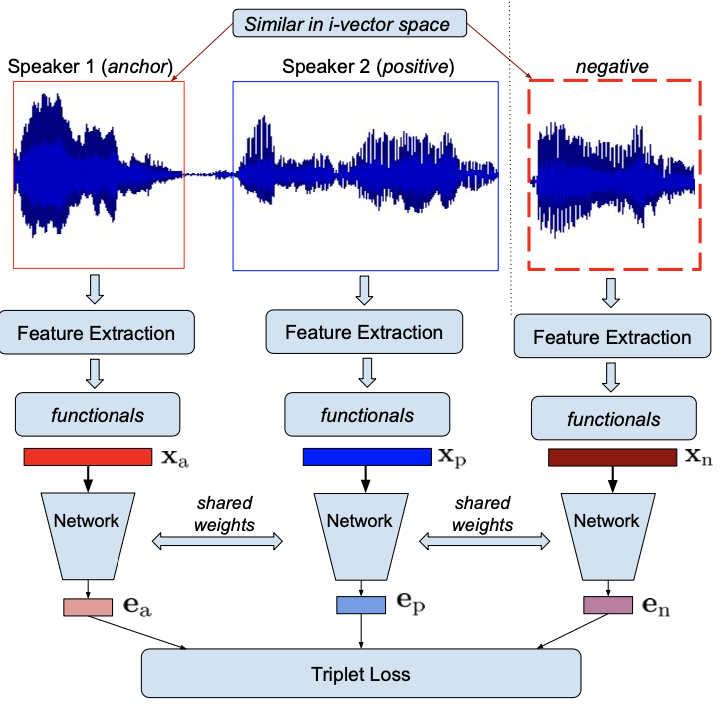
\includegraphics[width=0.6\textwidth]{images/triplet-model.png}
    \label{fig:sentiment_model_schematics}
    \end{sidecaption}
    \end{figure}

    We will utilize the following data and labels from Study-3:
            \begin{itemize}               
                   \item Audio recording
                    Transcript
                   \item Participant demographic information
                   \item Self-evaluation
                   \item MinecraftEntity\_Observation\_Asr\_Speechanalyzer
                   \item MinecraftEntity\_Observation\_Audio\_Speechanalyzer
                   \item MinecraftEntity\_Event\_Dialogue\_Event\_Dialogagent
            \end{itemize}
        % \item Our objectives (in decreasing order of priority):
        %     \begin{itemize} 
        %         \item Build a working statistical model for assessing entrainment while utilizing the vocalic features extracted by the ToMCAT-speechanalyzer system.         
        %         \item Train an encoding-based model using the methodology outlined in \textcite{nasir2020} for a simple classification task that identifies entrainment and directionality in a given conversation.
        %         \item Assess if the current Speechanalyzer system is set up to study entrainment trends as a time series. 
        %     \end{itemize} 

\section{Evaluation}

    Assessing entrainment involves calculating a similarity (or dissimilarity) measure between two utterances from the entrainment category, and observing if this metric of similarity increases or decreases as the speakers continue communicating. For this objective, accuracy scores for the classification task outlined above will be used to measure the performance of the entrainment detector. Because ASIST-ToMCAT is a multi-party conversation, we will examine the process of setting up new baselines for entrainment detection that can account for differences in team dynamics, reflected in how much each speaker talks, and how much other speakers respond to them.  

    We will also explore methods to evaluate two types of entrainment:

    \begin{itemize}
        \item Localized entrainment: Are there observable similarities between utterances by different speakers that occurred next to each other than utterances at different points in time?
        \item Global entrainment: after a given period of objective-oriented speech, is the speech from the conversation aligned more closely? 
    \end{itemize}

    In order to account for ASR errors in the automatically generated transcripts, we will create a corpus of human-generated gold transcriptions. From this corpus, a subsection of the data will be used to identify utterances separated by 50ms pauses, in order to assess any differences in performances due to ASR issues. A manual evaluation of the speech data will also be conducted to examine other environmental noise, so as to account for qualitative differences between the recording conditions of the pristine training data and the real-time ToMCAT speech data. 

   \section{Other Qualitative Assessments}

   Since speech entrainment in conversational setups is a feature of speaker bonding and closeness, it is useful to assess if it co-occurs with positive emotions in spoken statements, lower stress, and higher confidence in the plan and team actions in a co-operative goal-oriented setting. We will utilise the human-generated gold transcriptions as well as manual annotations for emotion and dialogue acts to qualitatively assess if entrainment co-occurs with positive emotions and the acts of sharing information, as well as the relationship between global entrainment and levels of stress and uncertainty. We will also examine if the directionality of entrainment (towards or away from any of the participants) is affected by members' personality or socio-cultural differences, in order to account for natural differences known to impact conversation styles.


\chapter{Online multi-agent plan recognition}
\label{ch:plan_recognition}
\textbf{Loren Champlin, Salena Ashton, Liang Zhang, Clayton Morrison}

\section{Introduction}

Plan recognition is the ability to understand and recognize logical structures and patterns within a sequence of observed behavior. Developing this capability for our AI agent would allow it to infer the latent plan structures, strategies, and goals (i.e., ``plan explanations") of not only individual human agents but a team of agents as well. Producing these plan explanations contributes to the logical belief structures that the AI agent must maintain as part of its theory of mind and theory of teams \citep{Tambe_1997,Baker_Tenenbaum_2014}. Furthermore, an AI agent could use these inferred plan explanations to predict the teams' subsequent actions and to help develop potential interventions for increasing team performance. Our AI agent must recognize the conjoined plan explanations of multiple agents given our team search and rescue setting and demonstrate this capability online (i.e., as the team carries out their mission). While a highly sparse topic, there are a few existing "state of the art" approaches for online Multi-Agent Plan Recognition (MAPR). 

The most recent online MAPR approach by \citet{Argenta_Doyle_2017} uses an automated planner to produce feasible plan explanations by simulating potential sets of parameters, conditions, and plan structures needed to generate the observed behavior. Approaches of this type are known as \textit{plan recognition as planning approaches} \citep{Ramirez_Geffner_2009,Van-Horenbeke_Peer_2021}. The use of an automated planner requires constructing a symbolic representation of the problem domain in which MAPR is to be deployed, known as knowledge engineering. Plan recognition as planning approaches are typically highly expressive and are capable of solving plan recognition problems that involve high levels of logical reasoning. However, this high expressivity usually comes at the cost of the high computational complexity required by the automated planner \citep{Van-Horenbeke_Peer_2021}. \citet{Argenta_Doyle_2017} attempt to overcome this challenge by making several strict simplifying assumptions about their problem domain. Although, these assumptions reduce the computational complexity at the cost of expressivity (i.e., it limits the type of problems their approach can solve). Another limitation is that \citet{Argenta_Doyle_2017} only consider ``flat" knowledge representations, rendering their approach incapable of inferring more than just the end-goals that the agents are trying to achieve. However, human behavior tends to exhibit hierarchical structures or patterns such that simple actions are combined to produce more complex actions. In terms of having a complete theory of mind and theory of teams, an AI agent needs to understand how actions relate to each other at different levels of granularity and complexity, not just how they relate to the agents' end-goals. 

Our proposed method for online MAPR is also a \textit{plan recognition as planning} approach. Rather than make assumptions that limit the problems our approach can solve, we try to overcome the challenges of computational complexity by developing a highly efficient automated planning algorithm specialized towards doing online MAPR. Our automated planning algorithm combines the well-known Simple Hierarchical Ordered Planner (SHOP2) proposed by \citet{Nau_2003} and the Monte Carlos Tree Search (MCTS) single-agent plan recognition algorithm proposed by \citet{Kantharaju_Ontanon_Geib_2019}. We also draw heavy inspiration from known parsing algorithms for Probabilistic Context-Free Grammars (PCFG) \citep{Collins_2011}. As suggested by its partial adaption of the SHOP2 algorithm, our approach assumes that the agents' actions relate through a set of hierarchical structures or what is known as a hierarchical task network (HTN) \citep{Nau_2003,Russell_Norvig_2021}. As such, our approach produces the most likely task hierarchy, which is an instance of a HTN under specific initial conditions. These task hierarchies represent how actions relate to each other at different levels of granularity of complexity by showing how high-level actions (also known as compound tasks) can be decomposed into low-level actions. 

\section{Approach}
In a HTN domain representation, compound tasks are high-level actions that are composed of lower-level actions. These lower-level actions may be compound task themselves that need to be further decomposed or non-decomposable actions, which are sometimes referred to as primitive tasks or just actions \citep{Russell_Norvig_2021}. Depending on how abstractly a compound task is defined, there may be multiple sets of lower-level actions that could be combined to create the same compound task. These different sets of actions are known as ``methods", since they are different ways of decomposing the compound task \citep{Russell_Norvig_2021}. Additionally, methods typically have preconditions, which are specific conditions that must be satisfied by the current state of the problem domain for that method to be used for task decomposition. If a methods preconditions are satisfied, then that method is said to be applicable \citep{Russell_Norvig_2021}. Figure \ref{pr_fig:1} further illustrates the concepts of compound tasks, actions, methods, and task decomposition. In the illustration, both methods could applicable or only one of them could be applicable given the current state of the problem domain. In the former case, an automated planner must choose one of the methods for decomposition, leading to two different possible plans. Further details on HTN planning processes can be found in the automated planning literature. (e.g., the SHOP2 paper by \citet{Nau_2003}). 

\begin{figure}[h]
    \centering
    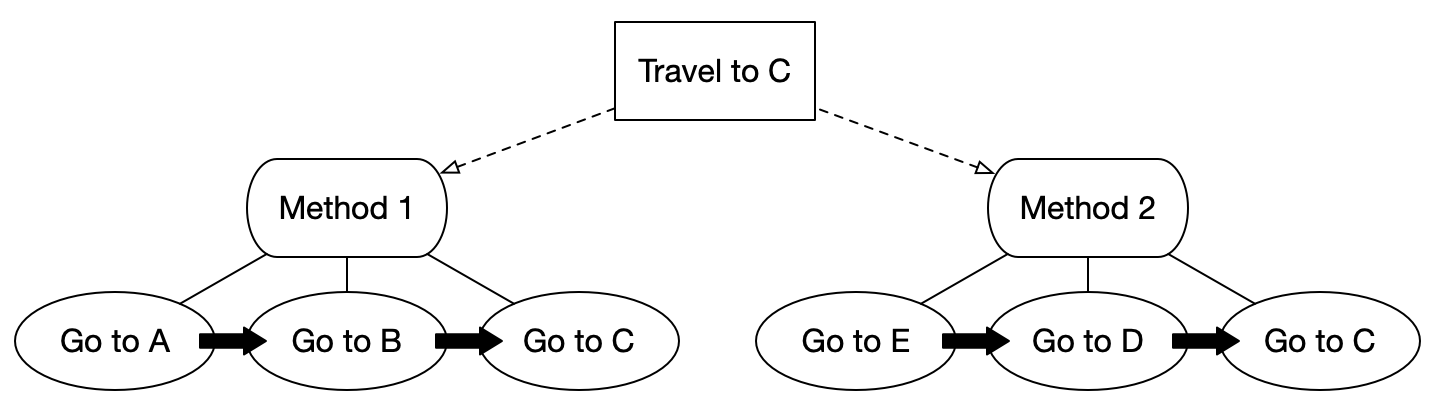
\includegraphics[width=1\textwidth]{images/htn_concepts}
    \caption{The compound task \textit{Travel to C} is shown to have two different methods for accomplishing the same task.} 
    \label{pr_fig:1}
\end{figure}

Our approach uses a HTN domain representation and an automated HTN planner to model the logical reasoning and decision-making process of a team of human agents. Compound tasks and methods are engineered in such a way as to represent the latent decisions that agents must make to complete their mission. From a generative perspective, these latent decisions are then what leads to the actions we observe from the human agents. With this concept in mind, we can have an automated planner generate a plan that matches the observed actions while recording the methods and task decompositions involved. As suggested in the introduction, this record is produced in the form of a task hierarchy which shows how compound task can be decomposed into the actions we observe. These task hierarchies are the plan explanations that give insight on the relationship between actions and the decision-making process of the agents. Figure \ref{pr_fig:2} illustrates the general concept of our online MAPR approach.

\begin{figure}[h]
    \centering
    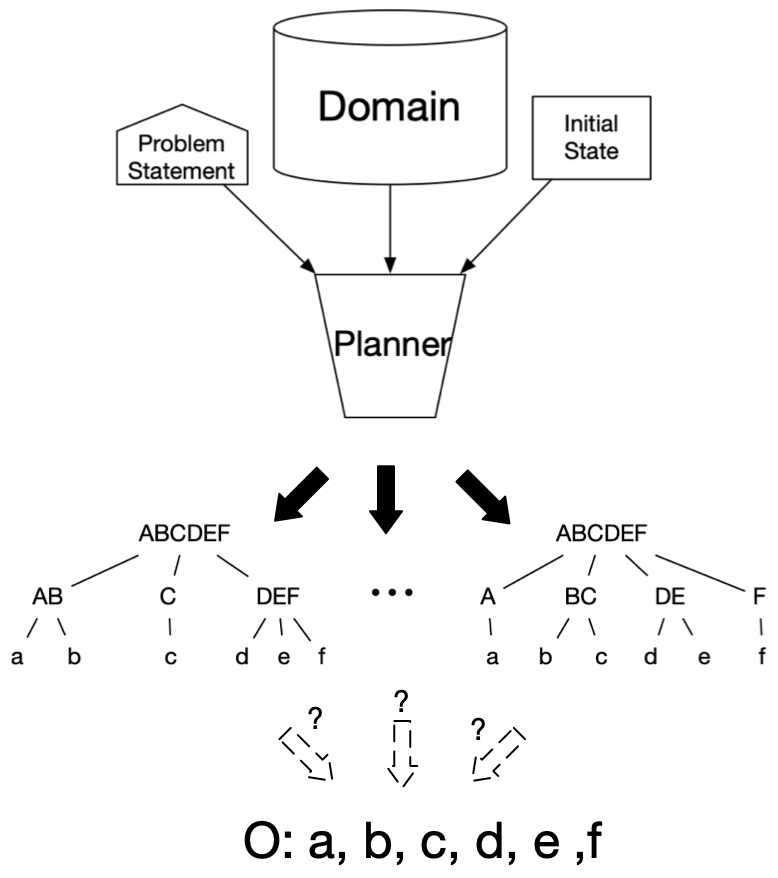
\includegraphics[width=1\textwidth]{images/pr_as_planning}
    \caption{In this illustration compound task are represented as groups of upper-case letters and actions are singular lower-case letters. Multiple potential task hierarchies can be generated for the same observed plan.} 
    \label{pr_fig:2}
\end{figure}

As seen in figure \ref{pr_fig:2}, it is possible that there are multiple plan explanations for same observed actions. However, rather than obtain all potential plan explanations given an observed sequence of actions, our approach should be yielding the most likely plan explanation. With this in mind, our approach assigns a conditional probability $p(m | \bigcap_{n \in M_t} c_n(s), s)$ for a method $m \in M_t$ for a compound task $t$. $c_n(s)$ denotes a function that is 1 if $n \in M_t$ is applicable to $t$ for the current state $s$, and 0 otherwise. The conditional probabilities are then defined as,

\begin{equation} \label{pr_eq:1}
p(m | \bigcap_{n \in M_t} c_n(s), s) = \begin{cases} \alpha  & c_m(s) = 1 \\ 0 & c_m(s) = 0 \\ \end{cases}
\end{equation}

\begin{equation}  \label{pr_eq:2}
\sum_{m \in M_t} p(m | \bigcap_{n \in M_t} c_n(s), s) = 1
\end{equation}

The value denoted by $\alpha$ in (\ref{pr_eq:1}) of each conditional probability must be predefined. As part of our approach we have formulated a training algorithm for learning these conditional probabilities, however that training algorithm is not detailed here. 

As suggested, an automated planner uses the methods defined in a HTN domain representation to decompose a compound task or set of compound tasks into a plan. This derivation of a plan is an analogous process to deriving a sentence from a PCFG. A PCFG contains a vocabulary of both non-terminal symbols and terminal symbols, as well as a set of derivation rules for replacing non-terminal symbols with a sequence of both non-terminal and terminal symbols \citep{Collins_2011}. Given an initial non-terminal symbol and applying rules successively eventually yields a sequence of only terminal symbols (i.e., a sentence) \citep{Collins_2011}. Similar to the methods of our HTN domain representation, each derivation rule is assigned a probability. Thus, given a specific derivation of a sentence (i.e., a specific set of derivations rules used), the probability of that derivation is the product of the probabilities of each rule used \citep{Collins_2011}. Given the similarities, we define the probability of a specific task hierarchy for a given plan in the same way. We denote $m_t$ as the applicable method chosen to decompose task $t \in \tau_\pi$, where $\tau_\pi$ is a set of tasks representing some task hierarchy used to generate a plan $\pi$. Using (\ref{pr_eq:1}), we have that,

\begin{equation} \label{pr_eq:3}
p(\tau_\pi) = \prod_{t \in \tau_\pi} p(m_t | \bigcap_{n \in M_t} c_n(s_t), s_t) 
\end{equation}

$s_t$ is current state prior to the decomposition of task $t$. Since our approach is for online MAPR, we want our plan explanations to consist of a partial task hierarchy that shows how the agents' latent decisions generates their plans up to the current time step. We denote the agents' observed partial plan (i.e., their observed sequence of actions up to some current time step) as $\pi^*$. We then simply replace $\pi$ in (\ref{pr_eq:3}) with $\pi^*$ to get,

\begin{equation} \label{pr_eq:4}
p(\tau_{\pi^*}) = \prod_{t \in \tau_{\pi^*}} p(m_t | \bigcap_{n \in M_t} c_n(s_t), s_t) 
\end{equation}

Using (\ref{pr_eq:4}), the objective of our approach is then to compute 

\begin{equation} \label{pr_eq:5}
\hat{\tau}_{\pi^*} = \argmax_{\tau_{\pi^*} \in T_{\pi^*}} p(\tau_{\pi^*})
\end{equation}

In (\ref{pr_eq:5}), $T_{\pi^*}$ denotes the set of all partial task hierarchies that match the observed partial plan $\pi^*$.

SHOP2 uses a depth first search (DFS) algorithm to generate plans and as such we could modify it to generate $T_{\pi^*}$ and then compute $\hat{\tau}_{\pi^*}$ by comparing $p(\tau_{\pi^*})$ for all $\tau_{\pi^*} \in T_{\pi^*}$ \citep{Nau_2003}. This is however an extremely computationally complex procedure and not a feasible method, especially for online MAPR where we would need to run this same computation many times. In general, using any automated planning algorithm to generate $T_{\pi^*}$ is not feasible. 

We argue that reasonable method would be to instead sample partial task hierarchies from $T_{\pi^*}$ and estimate $\hat{\tau}_{\pi^*}$ instead, this estimate being denoted $\bar{\tau}_{\pi^*}$. \citet{Kantharaju_Ontanon_Geib_2019} had come to this same conclusion in their development of an approach to do single-agent plan recognition using a domain representation based on Combinatory Categorical Grammars (CCGs). As mentioned in the introduction, they use a MCTS algorithm to sample the space of plans and find a reasonable estimate of the most likely plan explanation for an observed plan, reducing the computational complexity of their approach significantly. Using a similar concept, we modified the SHOP2 algorithm to use a MCTS algorithm as opposed to DFS. Although we will not go into full details here, MCTS samples solutions from the search space, which in our case are partial plan hierarchies matching the agents' observed partial plans. The search algorithm uses each sample to compute statistics about the search space that inform it where ``good" areas of the search space are according to some utility function \citep{Browne_Powley_Whitehouse_Lucas_Cowling_Rohlfshagen_Tavener_Perez_Samothrakis_Colton_2012,Kantharaju_Ontanon_Geib_2019}.In our case, our utility function is $p(\tau_{\pi^*})$, which the algorithm attempts to maximize. MCTS balances its search between completely unexplored areas and areas of the search space that have yielded good results before \citep{Browne_Powley_Whitehouse_Lucas_Cowling_Rohlfshagen_Tavener_Perez_Samothrakis_Colton_2012,Kantharaju_Ontanon_Geib_2019}. Given enough search time, our MCTS algorithm will eventually compute $\hat{\tau}_{\pi^*}$, although the needed search time would be roughly equivalent to what SHOP2 would need to do the same task. Therefore we must limit the search time allowed and have our algorithm return the best $\tau_{\pi^*}$ it can find under a predefined search time, which is our estimate $\bar{\tau}_{\pi^*}$. There is a high chance that $\bar{\tau}_{\pi^*}$ may only be a local optima, but it is likely to be a sufficiently probable plan explanation given a reasonable amount of search time. 

In terms of the Study 3 data, our approach heavily utilizes the json mission event messages coming from the message bus during the Search and Rescue mission trials. These messages are primarily used as the observations for our plan recognition algorithm, but are also used along with the video of the trials as source material for knowledge engineering our HTN domain representation. We also use the messages in our training algorithm to learn the conditional probabilities as defined in \ref{pr_eq:1} and \ref{pr_eq:2}. The specific input variables that we use in our approach from the message bus are as followed, 

\begin{itemize}
\item MinecraftEntity\_Event\_Triage\_Simulator
\item MinecraftEntity\_Event\_Roleselected\_Simulator
\item MinecraftEntity\_Event\_Proximityvictiminteraction\_Simulator
\item MinecraftEntity\_Event\_Playerfrozenstatechange\_Simulator
\item MinecraftEntity\_Event\_Tooldepleted\_Simulator
\item MinecraftEntity\_Event\_Markerplaced\_Simulator
\item MinecraftEntity\_Event\_Markerremoved\_Simulator
\item MinecraftEntity\_Event\_Markerdestroyed\_Simulator
\item MinecraftEntity\_Event\_Victimpickedup\_Simulator
\item MinecraftEntity\_Event\_Victimplaced\_Simulator
\item MinecraftEntity\_Event\_Rubbleplaced\_Simulator
\item MinecraftEntity\_Event\_Rubbledestroyed\_Simulator
\item MinecraftEntity\_Event\_Victimnolongersafe\_Simulator
\item MinecraftEntity\_Event\_Missionstate\_Simulator
\item MinecraftEntity\_Event\_Location\_Locationmonitor
\item MinecraftEntity\_Event\_Victimsexpired\_Simulator
\item MinecraftEntity\_Observation\_State\_Simulator
\item MinecraftEntity\_Observation\_Fov\_Fovtool
\item MinecraftEntity\_Event\_Dialogue\_Event\_Dialogagent
\end{itemize}

\section{Evaluation}
Since it would be extremely difficult to objectively confirm a teams latent decision process used for a mission trial, we have devised an alternative evaluation method for testing the performance of our online MAPR approach. The algorithm described in our approach section, can be reconfigured to project forward in time past the agents' observed partial plan, effectively allowing it to predict their most probable next actions using $\bar{\tau}_{\pi^*}$ as a reference point for the agents' latent decision-making process. We reason that the closer $\bar{\tau}_{\pi^*}$ is to the true value, the more accurate the action prediction will be. Using this concept, we can indirectly measure how well our approach works by measuring how accurate the action predictions are given $\bar{\tau}_{\pi^*}$.

While our algorithm could technically project forward to the end of a team's mission trial, we expect the prediction accuracy to increasingly diminish as the gap between the end of the projected plan and the observed partial plan increases. Instead we evaluate our algorithms performance by having it use $\bar{\tau}_{\pi^*}$ to predict only the next few actions. Given an observed plan from a completed mission trial, we can simulate having a teams' observed partial plan at a set time points in their mission. At these set time points, we can run our online MAPR algorithm and then have our planner predict the next few actions, and compare these predicted actions against the teams' true actions. 

We will compute two different types of accuracy measures, the action allocation accuracy and the action sequence accuracy, which are accuracy measures used in other MAPR literature \citep{Kim_Chacha_Shah_2015}. The action allocation accuracy is the ratio of how many predicted actions were correct out of the number of actions predicted \citep{Kim_Chacha_Shah_2015}. The action sequence accuracy is computed by first dividing the correctly predicted actions into pairs and then counting how many pairs are in the correct order (regardless of what actions they are predicted to have between them). This count is divided by what the count would be if all pairs were correctly ordered \citep{Kim_Chacha_Shah_2015}. The average action allocation and average action sequence accuracy over all trials will be computed for each prediction point, as well as average accuracy measures over all prediction points over all trials. 

We will also measure the rate at which our prediction accuracies decrease as we increase the number of actions predicted. This can be done by picking a singular prediction point for each trial and measuring the action allocation accuracy and action sequence accuracy as we increase the number of actions predicted. Increases in te number of actions predicted will be done at set intervals (e.g., 2 actions, 4 actions, 6 actions, etc).  Average accuracies will then be computed for each interval over all trials. 

\chapter{Probabilistic modeling of team coordination}
\label{ch:pgm}
\textbf{Paulo Soares, Kobus Barnard, Emily Butler}

\section{Introduction}
Human teams are interpersonal dynamic systems, where the individual team members
become subsumed by the collective whole in support of some shared goal or
function \citep{nowak2020insync, cooke2013Ainteractive, eiler2017interaction, fusaroli2014dialog, gorman2010team, wiltshire2017problem, wiltshire2019multiscale}.
All higher-order team behavior, such as cooperation or competition, emerges from
coordination, which refers to causal interdependencies over time both within and
between the individual team members \citep{butner2014modeling}. At the individual
level, there are a number of sub-processes within each person, such as biology,
attention, cognition, emotion and motor behavior that mutually influence each
other to give rise to the person’s overall state at a given time \citep{butler2011temporal,butler2017emotions}. Similarly, at the interpersonal level, the individuals interact with each
other to give rise to the team’s overall state \citep{nowak2020insync, butler2011temporal, butler2017emotions, cooke2013Binteractive, gorman2010team, letsky2008macrocognition}.

One challenge for predicting team behavior and outcomes is that coordination
within the system, at both individual and collective levels, often results in
non-linear state changes over time. For example, a team may be unsuccessfully
trying to reach an agreement until one member reframes the problem in a way that
suddenly broadens everyone’s perspective, leading to immediate group consensus.
The non-linear change in the team’s state of agreement could be predicted by the
first person’s increased mental coordination in their mapping of the problem
(increased within-person coordination), which colloquially might be described as
“having the pieces fall into place,” followed by the team’s increased group
coordination as all members adopt the new perspective (increased between-person
coordination). Thus being able to recognize ongoing changes in coordination (in
this example in the domain of mental contents) could help an artificially
intelligent agent predict subsequent non-linear changes in team states and
performance outcomes. 

One important aspect of social coordination is that it is not mode- specific
\citep{eiler2017interaction}. Instead, coordination can be observed at every level of
the system, including neural, physiological, motor, perceptual, cognitive,
affective and linguistic levels simultaneously. It can also be observed at
multiple time-scales \citep{wiltshire2019multiscale}. For example, during a
conversation, neural events transpire on the order of milliseconds, speech
production and gestures over seconds, and the conversation itself on the order
of minutes \citep{hasson2012brain}. As such, observing coordination for the
purpose of prediction should be possible at any time resolution and any
modality, although different modes will change at different rates and thus must
be assessed at different time resolutions. For example, during a conversation
coordination between the electrical activity of people’s brains may be best
observed in milliseconds, while coordination of the semantic content of their
speech may be best observed at the level of speech turns.

Social coordination has been operationalized in many ways, often with approaches
that are mode or time-resolution specific. We prefer a more general approach,
since the same representation can be used to index coordination for any aspect
of the interpersonal system, from individual brain activity to collective
behavior sequences. One advantage of this for developing a socially intelligent
artificial agent is that the agent can learn about coordination from any
available observable information, which has important real-world consequences
for how useful such an agent will be, since it will not be constrained to
situations similar to those in which it is developed. The fundamental concept
that needs to be captured by a general representation of coordination is the
predictive interdependencies over time among the components of the system. See
the “Modeling” section below for the details of our representation.

We also prefer measures that are easily interpretable. Although coordination
should be observable from any measure of the interpersonal system, some measures
will map more closely to intuitive domains of coordination than others. For
example, coordination of speech behavior is theoretically observable from any
derived measure of vocal signals during a conversation. Along these lines, work
with natural language processing has made use of dozens of automatically
extracted features from speech for categorizing a broad range of targets, such
as personality types or emotional expression \citep{eyben2010opensmile}. Although
successful categorization has been achieved using various subsets of the
features, it is unclear what aspect of human behavior contributed to the
results, making it impossible to go from the results to theoretically based
interventions. For the present research, therefore, we focus on coordination of
two vocal features that map directly to pitch and loudness of human speech (see
Methods for details), both of which could be targeted by an intervention as
simple as asking a person to speak softly. 

Finally, we also prefer models that are predictive and interpretable. XXXXXXX

\section{Hypotheses}
The proposed research will use data from ASIST Study 3, to be conducted in the Spring of 2022. Participants will take part in 3-person teams and will play a game where they attempt to save virtual victims in a Mindcraft Search and Rescue scenario. We will test the following hypotheses:

1) Including coordination as a node in a probabilistic graphical model
\textbf{will improve} prediction of team process and effect measures (see Measures for details)  as compared to a comparable model that does not include coordination.

2) Teams with higher coordination will have higher scores on measures of team process and effects (see Measures for details) than teams with lower coordination.

3) The agent has a set of three interventions to encourage oral communication among
team members. Teams where the agent intervenes will have higher coordination,
and higher scores on measures of team process and effects (see Measures for
details), than teams where the agent does not do this. For teams selected for
intervention will get interventions contingent on activities and also on how
many interventions have been done so far to avoid intervening too much.  The
interventions are:
\begin{enumerate}
    \item
    If a team member places a marker block (a form of communication provided in
    the game) but does not say they did, then the agent will suggest that they
    tell their team members that they placed it. 
    \item
    For some teams, if a team member needs help (to stabilize a victim or exit a
    blocked room) but does not say they do, then the agent will suggest that
    they tell their team members that they need assistance. 
    \item
    For some teams, if a team member asked for help but did not get a reply from
    any of the other team members, then the agent will suggest that they tell
    the others again that help is needed. 
\end{enumerate}

\section{Approach}

\subsection{Design}
Our analyses to test Hypotheses 1 and 2 will make use of data from all of the
participants in the study (e.g., all possible between- and within- participant
conditions). As such, testing whether including coordination in the model
improves prediction of team process and effects measures (Hypothesis 1) and
testing the association between coordination and team process and effects
measures (Hypothesis 2) will each be based on 224 missions (8 conditions X 14
teams X 2 missions). Our analyses to test Hypothesis 3 will make use of data
from the ``No-Advisor” and ``UAZ-Agent” conditions, and so testing the effect of
our intervention (Hypothesis 3) will be based on 28 ``No-Advisor” control
missions (14 teams X 2 missions) compared to 28 ``UAZ-agent” intervention
missions (14 teams X 2 missions).

\subsection{Measures}
\textbf{Coordination indicators}. As discussed above, team coordination is
theoretically observable across modalities and time resolutions for all of the
components of the interpersonal system. Given the constraints of what will be
measured for ASIST Study 3, we will focus on two vocalic measures that are to be
provided in real-time (every 10ms) during the missions as indicators for
modeling linguistic coordination. The first, ``F0final\_sma" is the smoothed
moving average of fundamental frequency. It corresponds to a speaker’s pitch.
The second, ``wav\_RMSenergy\_sma" is the Root Mean Square energy measure, which
provides an estimate of the intensity of the sound, which correlates with what
humans perceive as loudness. 

\textbf{Team Process and Effects Measures}. We will include 5 team process
measures and 2 team effects measures, each taken from the full set of measures
that will be available for ASIST Study 3. This subset was chosen due to either:
1) having theoretical connections to coordination (i.e., synchronization,
coordinative communications, belief differences) or 2) involving the use of
markers for communication, which is the direct target of our intervention
(threat room and victim type communication), or 3) representing a global measure
of team effectiveness (score and error rate).

The team process outcome measures are:
\begin{itemize}
    \item
    ASI-M2 Synchronization (e.g., inter-subtask latency); \textbf{Measure}: Mean latency
    between subtasks of teamwork tasks per trial. Specifically, the mean latency
    between victim discovery and victim rescue computed as the average over all
    correctly rescued victims (time of delivery of victim to correct rescue site
    - time victim was discovered). Where time victim was discovered = the
    earliest (or minimum) of (1) Transporter signalling device for the room
    containing the victim, or (2) Medic completes stabilization of the victim.
 
    \item
    ASI-M5 Coordinative Communications; \textbf{Measure}: A quantitative characterization
    of the complexity of team communication using entropy in the dynamical
    system. Entropy is defined as the level of irregularity in the flow of
    communications between team members.(i.e., Team Communication Dynamics).
    Typical components of the measure are: (1) Intensity and distributions of
    team communications are calculated using calculations of over message
    frequency, duration, and intra-team variance. (2) Temporal patterns of team
    communications are captured using timestamped communication events and
    analyzed with recurrence quantification analysis.

    \item
    Rutgers Threat Room Communication AC; \textbf{Measure}: \% of threat rooms that had a
    threat room marker block outside its entrance at some point during the
    mission.  

    \item
    Rutgers Victim Type Communication AC; \textbf{Measure}: count of victim
    type marker blocks placed near the correct type of A or B victims.
    
    \item
    Rutgers Belief Difference AC; \textbf{Measure}: entropy of beliefs about victim
    distribution by comparing three models in which (1) players share
    information perfectly, (2) players don't share any information, and (3)
    players only share information via marker blocks.  
\end{itemize}

The team effects measures are: 

\begin{itemize}
    \item
    ASI-M1 ASI Utility (SAR game score) 
    \item

    ASI-M3 Error Rate; \textbf{Measure}: Percentage of
    subtasks of teamwork tasks that are completed per trial, measured as below.
    Specifically, the percentage of discovered victims who are not evacuated.
    Measure = 1 - (\# victims rescued / \# victims discovered)
\end{itemize}

\subsection{Modeling}
    We develop a probabilistic model for measurement outcomes. In addition to
    reflecting an explanatory story, a key property of this approach relevant to
    evaluation as discussed below is all estimates are probability
    distributions. In needed, these can be distilled into point estimates by
    either averaging the distribution (MMSE loss) or using the maximum (MAP
    loss). 

    Our probabilistic model for this experiment (see  Figure~\ref{fig:pgm})
    models outcome measures, $M^i$, conditioned on a coordination latent construct, $C$. 
%
    \begin{figure}
    \label{fig:pgm}
    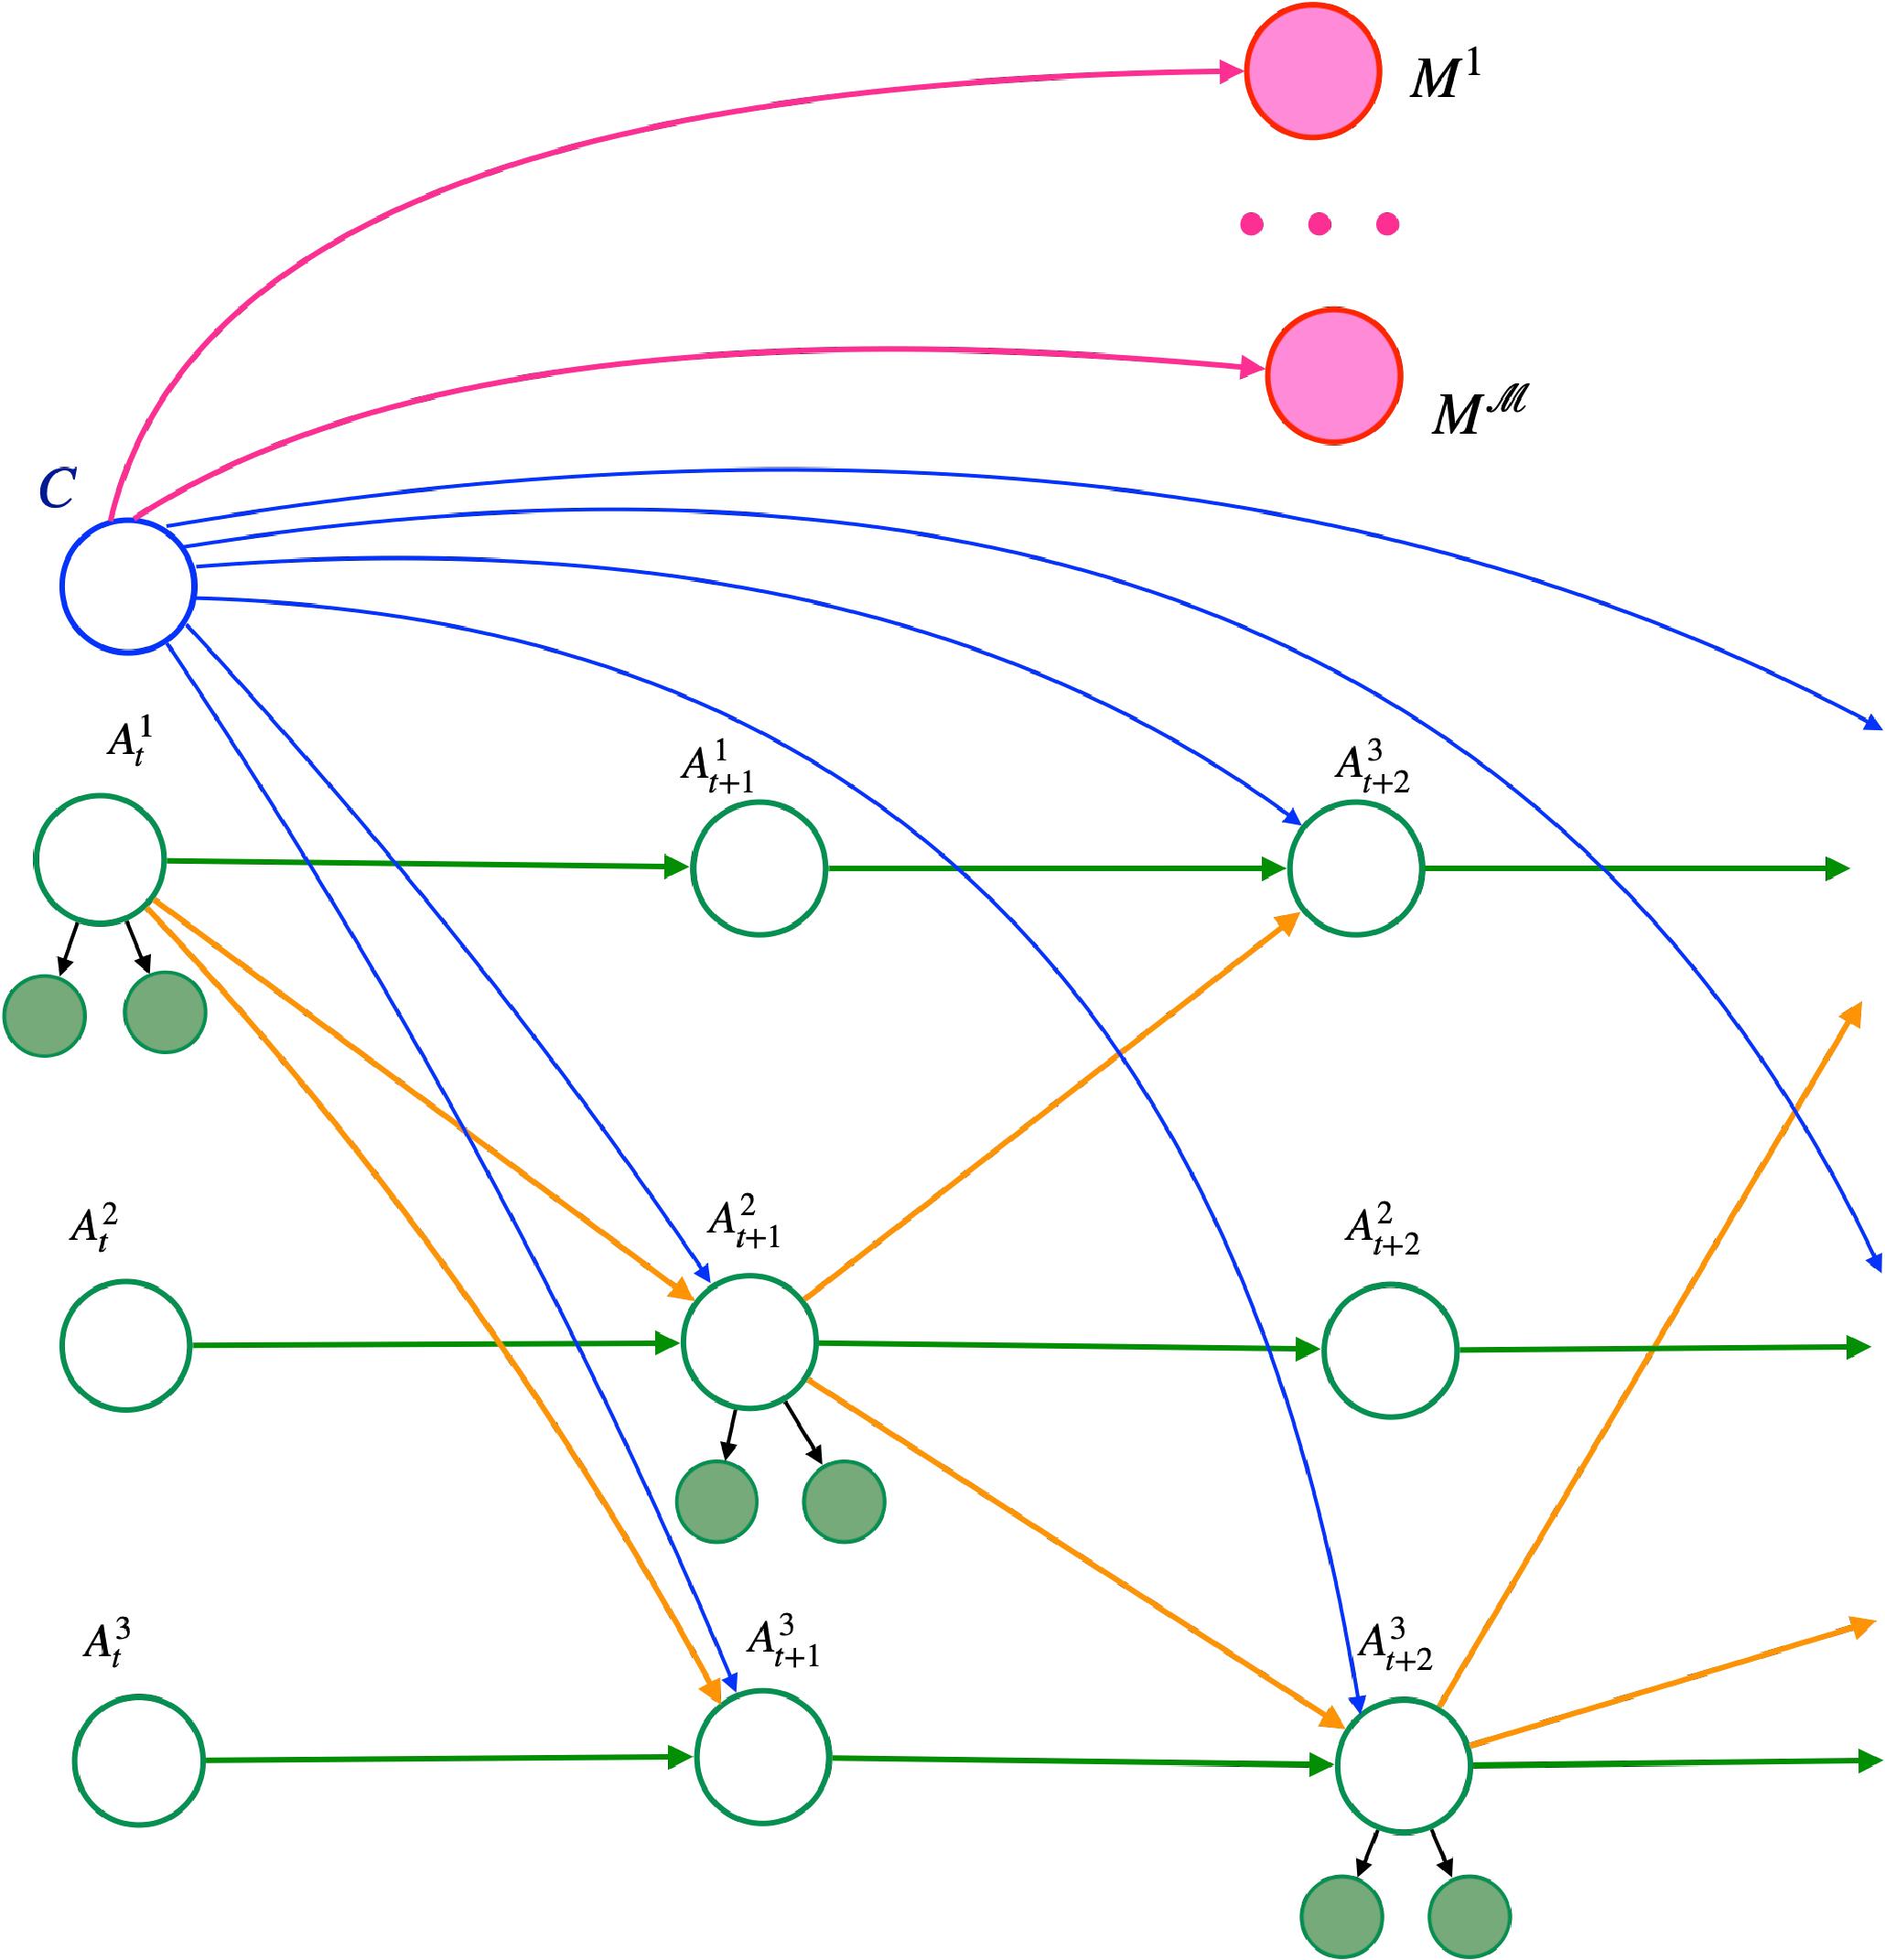
\includegraphics[width=6in]{images/prereg-pgm.pdf}
    \caption{Probabilistic graphical model (pgm) for investigating coordination.
    Circles (nodes) are stochastic variables. 
    Open circles are latent variables, shaded circles are potentially observed
    variables, and arrows represent variables conditioned on parents.
    Coordination, $C$, is posited to influence team efficacy measures, $M^i$.
    We do not use plate notation here because the conditioning arrows are
    measure specific). These are different linear functions learned from data with potentially
    different emission distributions (e.g., normal or Poisson), depending on the
    measurement construct. \\
    $~~~~~~~~$ Coordination is exhibited by variables influencing other variables in the
    next time step. We do not draw all possible arrows here, because, for
    vocalics, we assume that all  such influence comes from the previous speaker.
    Here we illustrate person 1 speaking, followed by person 2, and then person 3.  }
    \end{figure}
%
    The distributions $p(M^i|C)$ are typically linear functions learned from data
    with normal or Poisson emission distribution. Using a simple prior on $C$,
    provides a baseline model.

    \textbf{Coordination.}
    We would like to study the effect of including coordination in this model.
    We are developing a comprehensive probabilistic model for coordination, with
    a simple case exhibited as part of Figure~\ref{fig:pgm}.  While in the
    general case coordination influences multiple diverse modalities at
    different time scales, here we consider a single time scale and two vocalic
    features.  Our underlying axiom is that higher coordination is associated
    with causally driven increased mutual information (statistical dependence)
    between relevant observed variables. Here we consider latent attributes for
    vocalic style for person $p$, denoted by $A^{p}$, which has as evidence,
    $O^{p,1}$, being the mean of normally distributed pitch of speech over a
    speech turn and similarly $O^{p,2}$ for speech intensity.  We further assume
    that the speech style of each person is only influenced by the previous
    speaker.

    If person 2 speaks after
    person 1, then the degree that their vocalic style follows that of person 1
    indicates coordination. Formally, we blend the non-coordinated distribution
    mean, $\mu^2_t$, for the second person, with the fully dependent mean,
    $\mu^1_t$, for the mean for the second person at time $t+1$ by
    \begin{equation}
    \mu^2_{t+1} = (1-c) \mu^2_t + c\mu^1_t ~.
    \end{equation}

    To pre-register a single approach, we model coordination as being
    constant for the second half of the second
    trial. This allows for the team to develop some rapport and interventions to
    have an effect. 

\subsection{Intervention}

The agent has a set of 3 interventions that were designed to encourage oral communication among team members. The interventions are

\begin{enumerate}
	\item \textbf{Marker Block:} the agent intervenes whenever a team member places a marker block, but do not let their team mates know about it.
	\item \textbf{Help Request:} the agent intervenes whenever a team member needs assistance, but do not ask for it.
	\item \textbf{Help Request Reply:} the agent intervenes whenever a team member asked for help, but any of the other team members replied.
\end{enumerate}

The agent uses a state machine to determine when to watch/monitor, activate or cancel a specific intervention. The general idea is illustrated in \ref{fig:intervention_state_machine}. Different events in the game might trigger different interventions and state transitions. These events and the rules associated with them are detailed in the following subsections and the list of topics the agent uses to detect these events and other relevant information about the missions are listed in Table \ref{tab:intervention_variables}.

\begin{table}
    \small
    \centering
    \begin{tabularx}{6in}{lp{1.2in}X}
        \toprule
        Topic & Publisher & Purpose\\
        \midrule  
    	trial & simulator & Determine a mission start and end \\
    	observations/events/mission & simulator & Determine the list of team members and mission order \\    
    	agent/dialog & UAZ Dialog Agent & Determined what relevant information was said by the team members \\
    	observations/events/player/triage & simulator & Determine interaction with a victim \\    
    	observations/events/player/victim\_picked\_up & simulator & Determine interaction with a victim \\
    	observations/events/player/marker\_placed & simulator & Determine a marker placement \\
    	observations/events/player/marker\_removed & simulator & Determine a marker removal \\  
    	observations/state & simulator & Determine the team members' positions \\	
    	observations/events/player/role\_selected & simulator & Determine the team member's role \\
    	observations/events/player/rubble\_collapse & simulator & Determine if an obstacle is blocking an exit \\
    	observations/events/player/tool\_used & simulator & Determine if an obstacle is being destroyed \\
    	observations/events/player/proximity & IHMC Proximity AC agent & Determine the team member's area \\
    	observations/events/player/rubble\_destroyed & simulator & Determine an exit was unblocked \\   
    	agent/pygl\_fov/player/3d/summary & FoV Tool & Determine objects in the team members' field of view \\    	
        \bottomrule
    \end{tabularx}
    \caption{%
        List of testbed message topics the agent is subscribed to.
    }
    \label{tab:intervention_variables}
\end{table}

\subsubsection{Marker Block}

The agent will start to monitor an intervention of this kind whenever a team member places one of the following markers:
\begin{itemize}
	\item Critical Victim
	\item Regular Victim
	\item Rubble
	\item SOS
\end{itemize}

These are the types that convey the need for other team members assistance. Therefore, it is important that the team knows when markers of these kinds are placed. 

Despite the fact that markers show up in the interactive map, the verbalization of a marker placement is essential to drive the team members' attention to the map as they might not be looking at the map at the time of placement. 

Once the agent starts to watch this intervention, it can either cancel or activate it depending on the next actions of the team member who placed the marker in the first place. If the intervention is activated, the agent will send a message to the team member who placed the marker with the following content

\begin{quote} 
    \centering 
    \emph{``[Player color], let your teammates know about the [marker type] marker you recently placed.''}
\end{quote}

The agent only intervenes once for each watched marker. This means that once the intervention gets activated, the agent removes it from the queue of watched interventions. The rules for switching to one state or another are detailed in the Figure \ref{fig:marker_block_intervention_flow_chart}.

\begin{figure}
    \centering
    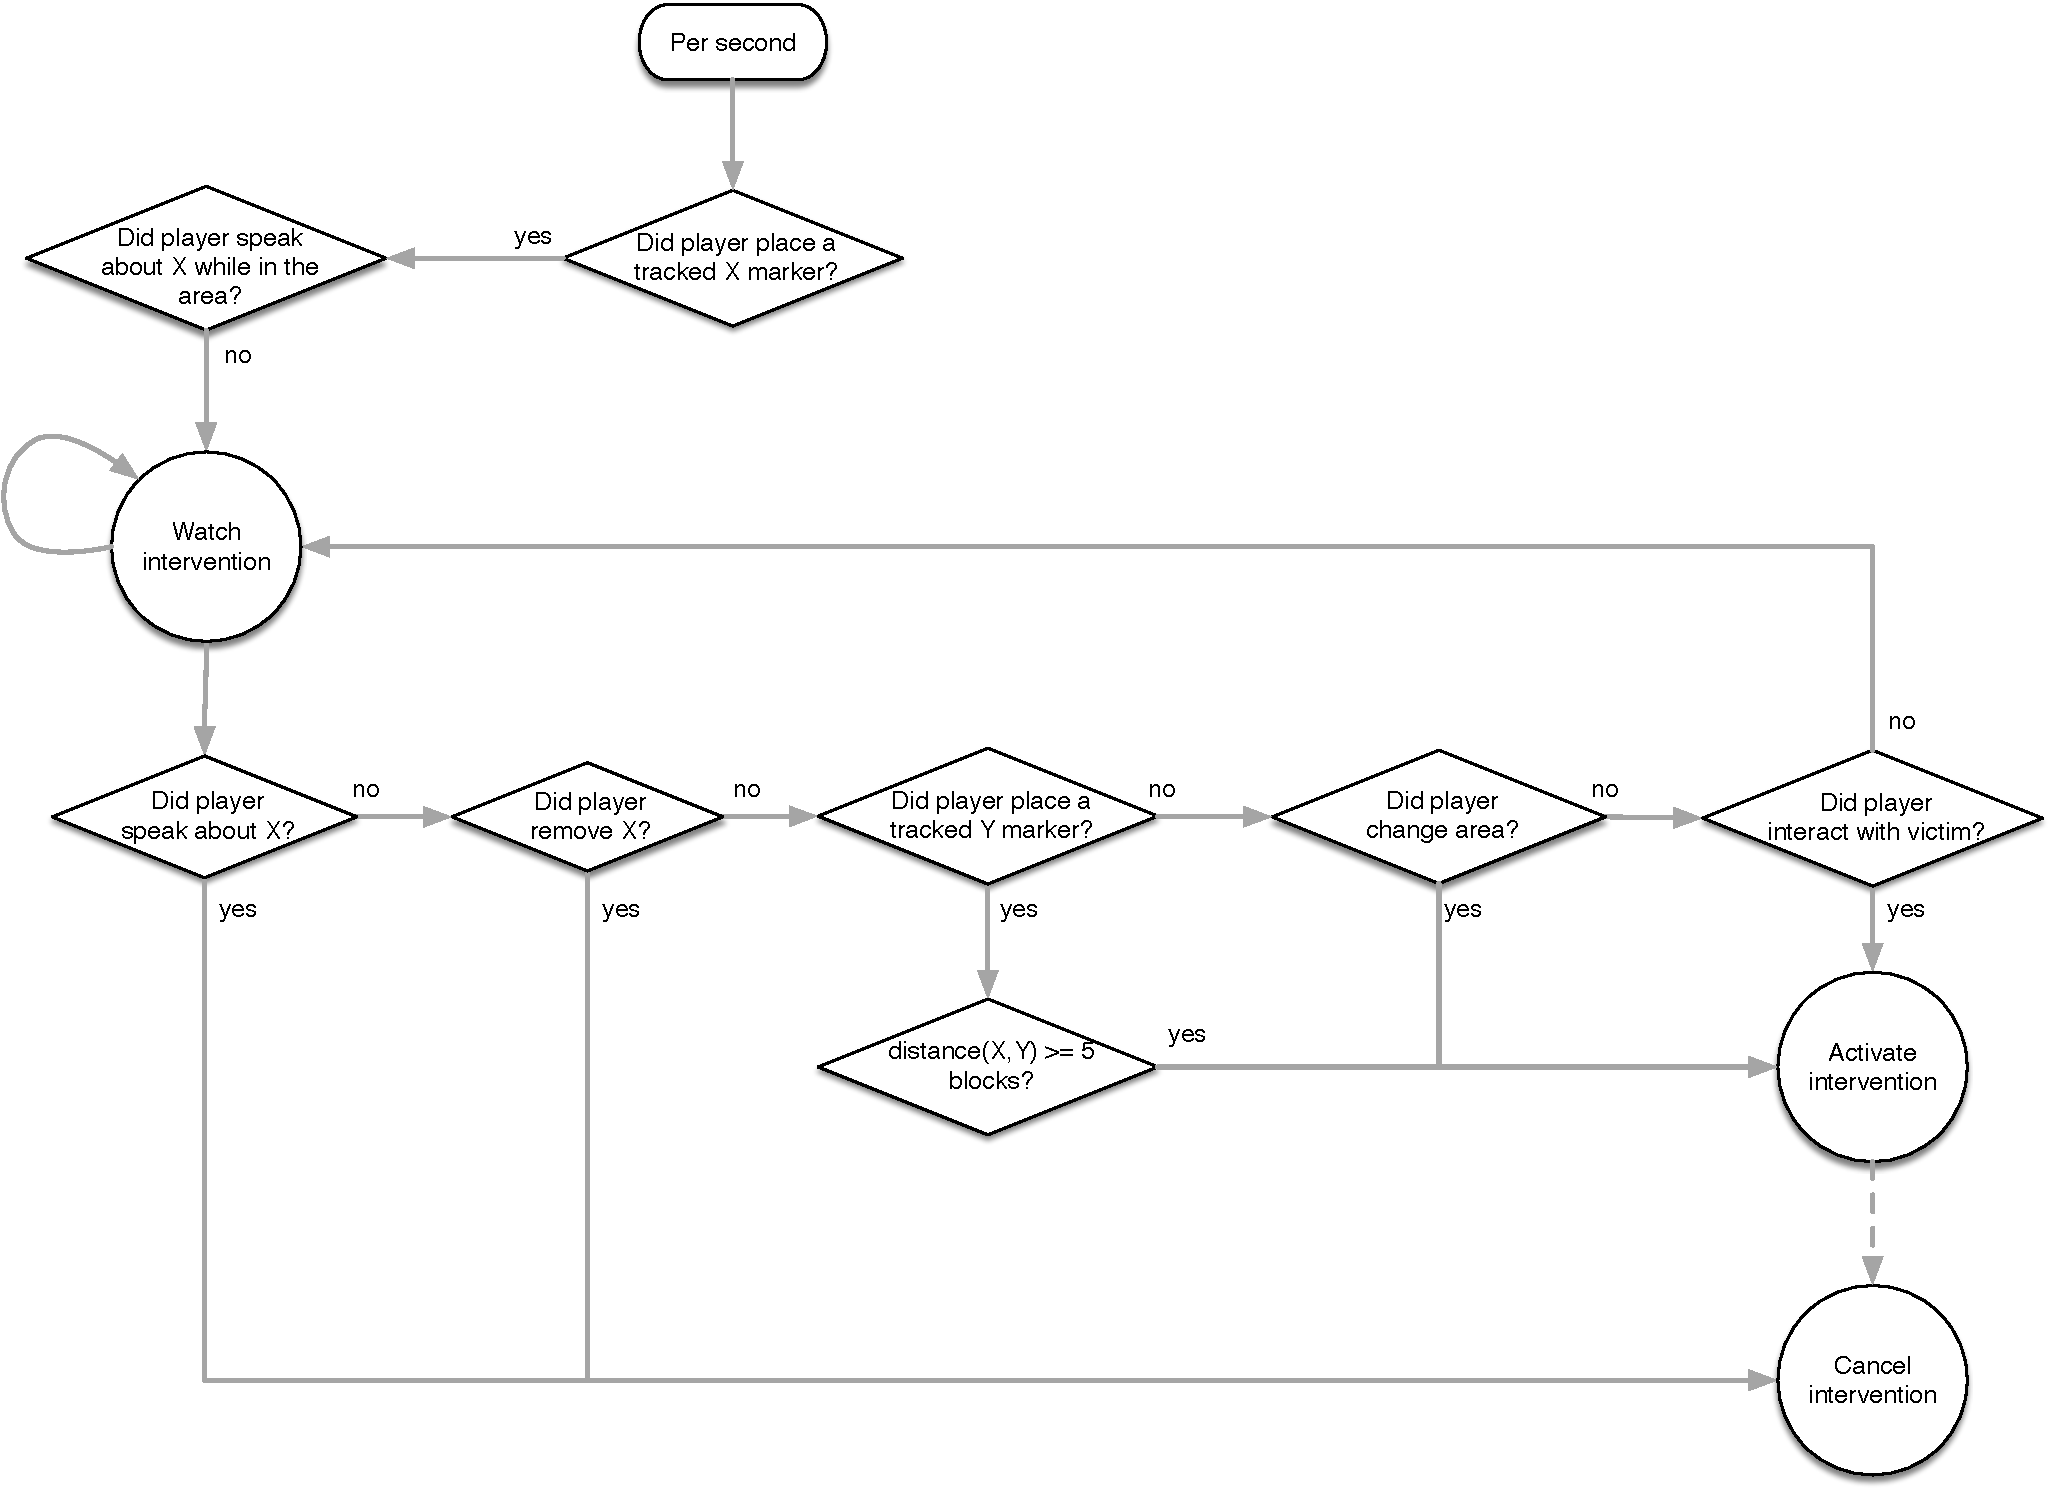
\includegraphics[width=6.5in]{images/marker_block_intervention_flow_chart.pdf}
    \caption{State transition rules for a marker-block intervention. This intervention gets activated whenever the team member that placed the original marker $X$ switches location in the map (e.g. from room A to room B), interacts with a victim (e.g. picks up a victim) or places another marker of different type or same type as X but far enough. The intervention is canceled if its objective is fulfilled or its object destroyed, that is, if the team member speaks about X or removes it respectively.}
    \label{fig:marker_block_intervention_flow_chart}
\end{figure}



\subsubsection{Help Request}

The agent will start to monitor for an intervention of this kind whenever a team member notices they are blocked inside a room or when they are close enough to a critical victim. These two events require team members to request assistance from others.

The agent considers a team member noticed rubble blocking their way out of a room if the obstructed exit is in the team member's field of view and within a range of 5 blocks from the team member's position. The same rule is applied for inference of critical victim perception. 

The activation or canceling of this intervention depends on the next actions taken by the team member that needs help and amount of time passed since the agent started to monitor this intervention. If the intervention is activated, the agent will send a message to the team member who needs help with one of the following contents

\begin{quote} 
    \centering 
    \emph{``[Player color], it seems you need some help to rescue a critical victim. Ask your teammates for assistance.''}
\end{quote}

\begin{quote} 
    \centering 
    \emph{``[Player color], it seems you need some help to exit this room. Ask your teammates for assistance.''}
\end{quote}

The rules for state transitions are illustrated in the Figure \ref{fig:help request_intervention_state_machine}.

\subsubsection{Help Request Reply}

The agent will start to monitor for an intervention of this kind whenever a team member asks for help. The agent detects when a team member asked for help by using the rule-based entity and event extractions \ref{ch:rule_based_ie}.

The transition to an active or canceled state, depends on the next actions taken by the team member that asked for help, subsequent utterances of other team members and amount of time passed since help was requested. If the intervention is activated, the agent will send a message to the team member who asked for help with the following content

\begin{quote} 
    \centering 
    \emph{``[Player color], it's been a while since you asked for help. Remind your teammates.''}
\end{quote}

State transition rules are detailed in the Figure \ref{fig:help request_reply_intervention_state_machine}.

\section{Evaluation}

\textbf{Hypothesis 1}: modeling coordination improves outcome prediction.  For
hypothesis 1 we train two different models (with and without coordination) on
the same training sets in the cross validation splits. We then apply that model
to held out data. The result in either case is a distribution for each outcome
variable. Given the actual value of the outcome variable treated as a real
number, we will evaluate predictive accuracy by using the mean of the
distribution (MMSE loss) compared to the actual value and compute the squared
error over all test splits in a leave one out cross validation scenario. For
completeness, for any categorical outcomes we would compare the value with
maximal probability with the observed one. 

\textbf{Hypothesis 2}: increased coordination predicts higher outcome scores.
Here we are interested in the learned model. In particular, we posit that the
slopes in the sub-models for the measures, i.e., $p(M^i|C)$ will be positive. We
will estimate the posterior distribution of those slopes over relevant data. The
mean and variance of that distribution will give some idea as to the validity of
the claim that coordination and a particular measure are positively correlated.
Sampling this distribution will reveal intervals that capture the probability
that this is valid within various ranges. 

\textbf{Hypothesis 3}: intervening on team communication predicts higher
coordination and SAR game scores. Here we have two distinct data cases. Each leads to
a probability distribution for coordination and score. Specifically, each run
contributes multiple samples to one of those distributions. We sample those
distributions to evaluate the hypotheses. Intuitively, it is easy to estimate
how often the statement is true ignoring the effect size, and the expected
difference, and the probability that it exceeds a desired value.  






% hypotheses?
% - TMM model can predict behavior
% - TMM agent interventions improve performance
% - Closed loop communication is predictive of team performance
\printbibliography
\end{document}
